\documentclass[11pt,journal,final,a4paper]{IEEEtran}
\IEEEoverridecommandlockouts
% The preceding line is only needed to identify funding in the first footnote. If that is unneeded, please comment it out.
\usepackage{cite}
\usepackage{amsmath,amssymb,amsfonts}
\usepackage{graphicx}
\usepackage{textcomp}
\usepackage[final]{pdfpages}
\usepackage[normalem]{ulem}
\useunder{\uline}{\ul}{}
\usepackage{xcolor}
%\usepackage[nolists,nomarkers]{endfloat}
\def\BibTeX{{\rm B\kern-.05em{\sc i\kern-.025em b}\kern-.08em
    T\kern-.1667em\lower.7ex\hbox{E}\kern-.125emX}}
\begin{document}

\title{Analyzing Topic Prevalence in Popular Hacker News Stories\\
}

\author{\IEEEauthorblockN{Jake J. Dalli} \\
\IEEEauthorblockA{\textit{Department of Artificial Intelligence} \\
\textit{Faculty of ICT}\\
University of Malta \\
jake.dalli.10@um.edu.mt}
}
\markboth{ICS5115 - Statistics for Data Scientists, MSc. Artificial Intelligence, SEM 2, ̃June 2019}{Shell \MakeLowercase{\textit{et al.}}: A Novel Tin Can Link}

\maketitle

\begin{abstract}
The online link aggregator Hacker News has emerged as one of the prime rallying points for startup founders, venture capitalists and technology workers; grasping the attention of this cohort of internet users carries intrinsic value. In this paper, we should how certain topics more likely to make it to the front page and that specific topics are definitely over-represented within the top post. We frame the problem as a topic mining challenge, applying a bayesian generative statistical model, Latent Dirichlet Allocation (LDA), and subsequently analyzing it to draw our conclusions.
\end{abstract}
\begin{IEEEkeywords}
Statistics, Machine Learning, Data Mining, News, Aggregator, Topic Mining, Latent Dirichlet Allocation, Natural Language Processing
\end{IEEEkeywords}

\section{Introduction}
Founded by venture capitalist Paul Graham in 2007, Hacker News (HN) is a news aggregator which lies at the heart of the startup renaissance\cite{hn:announcement}. While initially tailored towards startup founders, HN has come to represent more than just startup information, with participants urged to post \textit{"anything that gratifies one's intellectual curiosity."} In this paper, we perform an analysis of the front page with particular attention to the temporal and topical aspects of the data at hand\cite{hn:guidelines}.

Our results indicate that certain topics related to corporate revenue growth, such as making money, corporate transactions and recruitment; and topics related to programming niches such as Rust and Ruby programming, concurrency and parallel programming and interpreted languages tend to make it to the front page more often. We also conclude that posts related to web browsers tend to be over-represented within the top ranked story.

\section{Approach}
We aim to investigate the composition of the front-page of the aggregator, looking to understand whether any topics are particularly prevalent, and what other attributes a popular story might posses. Thus, we ask the following questions:
\begin{enumerate}
\item Is it easier to make it to the front page of Hacker News if you publish an article on a specific day or at a specific time?
\item Are there particular topics which make it more often to the front page?
\item Are some topics over-represented within the top post?
\end{enumerate}

The task of detecting topics lends itself towards the field of generative models, due to the fact that we are looking to generate a number of outcomes (in this case topics) based on our input observations\cite{lda:generative}. Moreover, we also consider that our problem domain may result in noisy or incomplete data. Apart from news articles, HN users also post links to videos,  unconventional web pages and web applications (this is particularly prevalent for stories tagged \textit{Show HN}) amongst others.

Our analysis takes two different forms; we first perform a \textbf{descriptive analysis} of the dataset, investigating the statistical relationship between points and comments, and the relationship between the date and time that the story was published in relation to the rank of the story; secondly, we perform \textbf{topic detection} by building a \textit{bayesian generative statistical model} to analyze the topics detected\cite{lda:bgsm}. 

With these goals in mind, we make two key assumptions by analyzing the hackernews datasource:
\begin{itemize}
\item We shall limit our analysis to the top 30 HN stories for a given day, ranked by the number of points the article received. This is distinctively different to analyzing the articles which appear on the front page. The HN front-page is composed both of top ranked articles, and new articles. Typically new articles quickly make their way out of the front page if they do not receive enough points to maintain their presence. Thus one key assumption is that the top 30 articles ranked by points have appeared on the front page. This assumption allows us to draw more accurate results by eliminating noise from the dataset. 
\item We limit our approach to detecting topics within text-based stories, purposefully excluding or knowingly disregarding stories which link to files (such as PDF documents), web applications or videos. Our approach only considers text articles. 
\end{itemize}

\subsection{Latent Dirichlet Allocation}
We approach the task of topic detection by building a generative model using \textit{Latent Dirichlet Allocation}, which represents documents as mixtures of latent topics characterize by term distributions \cite{lda:bengio-ng}. The model assumes the following process for each document $d$ in a corpus $C$:
\begin{enumerate}
\item Choose the number of terms $N$ assigned to a document according to a Poisson distribution $\phi$
\item Choose a topic mixture $\theta$ according to Dirichlet distribution $\alpha$ over a fixed number of $K$ topics. 
\item For each $N$:
\begin{enumerate}
\item First pick a topic $Z_{n}$ based on a multinomial distribution sampled from $\theta$.
\item Based on $Z_{n}$ generate a term $w_{n}$ from \\ 
$p(w_{n}|Z_{n},\beta)$, computing a multinomial probability conditioned on $z_{n}$

\end{enumerate}
\end{enumerate}

To illustrate this, consider a corpus containing documents about company transactions. A document headlined \textit{"Salesforce acquires Tableau for \$15.8B"} may yield the terms \textit{Salesforce, acquire, Tableau} ($N=3$). We may have two topics ($K=3$) about \textit{mergers, acquisitions and restructurings}. LDA would generate the three terms with their relative probability in relation to the topics; so for example the term $Salesforce$ would be associated to the three topics \textit{mergers, acquisitions and restructurings} with probabilities $P_{m} = 0.3$, $P_{a} = 0.9$ and $P_{n} = 0.5$ respectively. 

Given enough documents which outline several acquisitions by \textit{Salesforce}, we may discover a topic which specifically relates to company transactions by the company.

The LDA process assumes prior knowledge of the number of topics, $K$ which are to be detected. This can prove challenging in applications where the number of topics is not known a priori. Thus the LDA approach is tightly coupled with a parameter estimation problem for deducing the ideal number of topics. 

Topic mixture can be evaluated by computing the \textit{Maximum Log Likelihood} of the given data \cite{lda:evaluation}. This is done by holding out a test set of unseen documents $D_{t}$, to be evaluated against a topic matrix $\Upsilon$, with a hyper-parameter $\alpha$. Thus the Log-Likelihood can be computed as follows:
\begin{equation}
L(W) = log P(d | \Upsilon , \alpha) = \sum_{t} log P( d_{t} | \Upsilon, \alpha)
\end{equation}

One can thus measure the \textit{perplexity} of a topic model:
\begin{equation}
perplexity(w_{n..t}) = \begin{Bmatrix}
-\frac{L(W)}{Total  Tokens}
\end{Bmatrix}
\end{equation} 

There are some observations to be made when evaluating topic mixtures. Firstly, the concept of a topic is highly coupled to human reasoning which is not quantitatively justifiable, thus perplexity and model quality may not be correlated \cite{lda:human-perplexity}. Secondly, the \textit{Log Likelihood} calculation is prone to local maxima, thus one must adjust additional hyper parameters to skip or discard certain iterations.

\subsection{Data Collection and Storage}
The Hacker News interface is updated in real-time with no pages showing the history of story submission. Each story is accompanied by a story headline, story publish date, number of points and comments, story link, thread link and source domain.

We perform a one-time web page extract from the meta-aggregator HckrNews\cite{hn:datasource}, a website which displays an archive of the top voted HN stories by date and time. Our extract consists of the top 50\% of stories on the HN board for six months ranging from \textit{1st December 2018} till \textit{31st May 2019.} 
In turn, we design a pipeline of R scripts which extract the following data sources:
\begin{enumerate}
\item \textbf{List of Stories:} Parse the HTML page for stories, output a clean dataset with the aforementioned fields in comma delimited format (CSV). Filter out only the top 30 stories for each day by points.
\item \textbf{Source Pages:} For every story, visit the story link and download the web page in raw HTML format. This results in a repository of HTML pages accessed via the source link.
\item \textbf{Source Datasets:} Two datasets containing the stories extracted;  \textit{hackernews board}, containing only data shown on the bulletin board for the top 30 hackernews stories between 1st December 2018 and 31st May 2019; and \textit{hackernews board content} which additionally contains the corpora (source pages and story headline keywords) which we shall use for topic processing and analysis. We explain the steps for cleaning and aggregating such data within the subsequent section.
\end{enumerate} 

Our results are stored in a dataset called \textit{final-annotated-topic-document-matrix.CSV}, which contains every story and its probability of association to each one of the 114 detected topics. It also contains the topic meta-data for the topics with the top three probabilities.

\subsection{Data Preparation and Cleaning}
Our preparation and cleaning processes perform three functions; firstly we perform some superficial cleaning and preparation of the \textit{story list dataset}, by removing sub-strings related to website aesthetics. Secondly, we carry out information extraction on the source page HTML documents, to extract clean text from the HTML markup. Lastly, we perform a number of \textit{Natural Language Processing} preparation techniques on the extracted repositories to reduce the volume of the data, and refine the textual representation in order to render better results. 

The latter process proves to be nuanced, since it requires taking some strategic decisions to reduce the volume of data, and to remove linguistic features which may not be good ontological indicators. We assume that a document's ontological composition is adequately represented by its \textit{noun phrases} and \textit{verb phrases}. Another assumption is that the first 800 words of a document represents the ontological composition of a document, this is done to reduce the data volume. We also strip text corpora of punctuation and stop-words. Finally, we perform word stemming on the dataset. 

We make use of the \textit{BoilerpipeR R library}\cite{cran:boilerpiper} to detect and remove template code from the HTML pages, which provides a model specifically trained for extracting articles from news website templates; furthermore, we use the \textit{Text Mining and Open NLP} R libraries to clean the text data\cite{cran:textmining}\cite{cran:opennlp}. 

In summary, we perform the following processes on the data:

\begin{enumerate}
\item Extract the story name, points, comments, source domain, source link, thread link, rank and publish date from the HckrNews\cite{hn:datasource} archive:
\begin{itemize}
\item Remove the source domain from the story name.
\item Remove any trailing white-spaces
\item Convert the publish date to a readable date format.
\item Save the dataset as \textit{hackernewsboard.csv}
\end{itemize}
\item For every story, visit the source domain and download the HTML page to the source article repository.
\item For each story, read the relevant documents from the source page repository. Extract nouns and verbs from the story text and story headline and save to separate fields within the data frame. Save this dataset as \textit{hackernewscontent.csv}.
\end{enumerate}

\subsection{Methodology}
Our analysis takes two forms. Within our descriptive analysis, we aim to answer the following questions:
\begin{enumerate}
\item \textit{Is there a correlation between the number of points and the number of comments a story receives? Are some data sources more successful than others?} 
\item \textit{Does the time of day and day of week affect the ranking a story receives?}
\end{enumerate}

The second part of our analysis involves training a Latent Dirichlet Allocation Model trained on the extracted data. Our model is trained with a corpus containing of documents representing the \textit{Noun Phrases} and \textit{Verb Phrases} within the story headline, and the first 800 words of the source page.

We do this by constructing a Document Term Matrix (TF-IDF) and training the model using \textit{Gibbs Sampling} to find the conditional probability distribution of a word's topic assignment, modifying $\theta$ to achieve the maximum log likelihood. However, this method assumes that we already know the number of topics we need to detect.

Thus, we must perform a \textit{parameter selection process}, repeatedly running the model with different values of $K$, and evaluating the topic mixture by calculating the \textit{Maximum Log Likelihood.} Each model is run using 700 iterations, discarding the first 200 iterations to increase accuracy. The results for this process are reported within our analysis. 


When the ideal k is selected, we train our model once again to preform our analysis, answering the following questions:
\begin{itemize}
\item \textit{Are there particular topics which make it more often to the front page?} We build a document-topic probability correlation covariance matrix representing the correlation of two topics on our document. Next, we cluster the topics based on their covariance using hierarchical clustering. The clusters detected are indicative of groups of topics appearing more frequently on the front page.
\item \textit{Are some topics over-represented within the top post?} We create a bucket for the rank attribute, marked \textit{true} if the article is top ranked, and \textit{false} if the article has any other rank. Next, we perform a Chi Square Test\cite{test:chi} to investigate the correlation between a top ranked article and the topic. To ascertain our results, we also perform a One-Way ANOVA test\cite{test:anova} on the ranking as an ordinal value.
\end{itemize}

The primary method for topic detection used is Latent Dirichlet Allocation, as provided by the \textit{Topic Models R library}\cite{cran:topicmodels}; We visualize our data using the \textit{GGPlot R library}\cite{cran:ggplot}, using a theme derived from that produced by The Economist magazine. 


\section{Descriptive Analysis}
We begin our analysis by plotting stories and sources. The plots are densely populated at the zero axis, becoming less densely populated as they increase in points and comments. This is indicative of the fact that higher story rankings are more difficult to achieve.

\begin{figure}[!ht]
\centerline{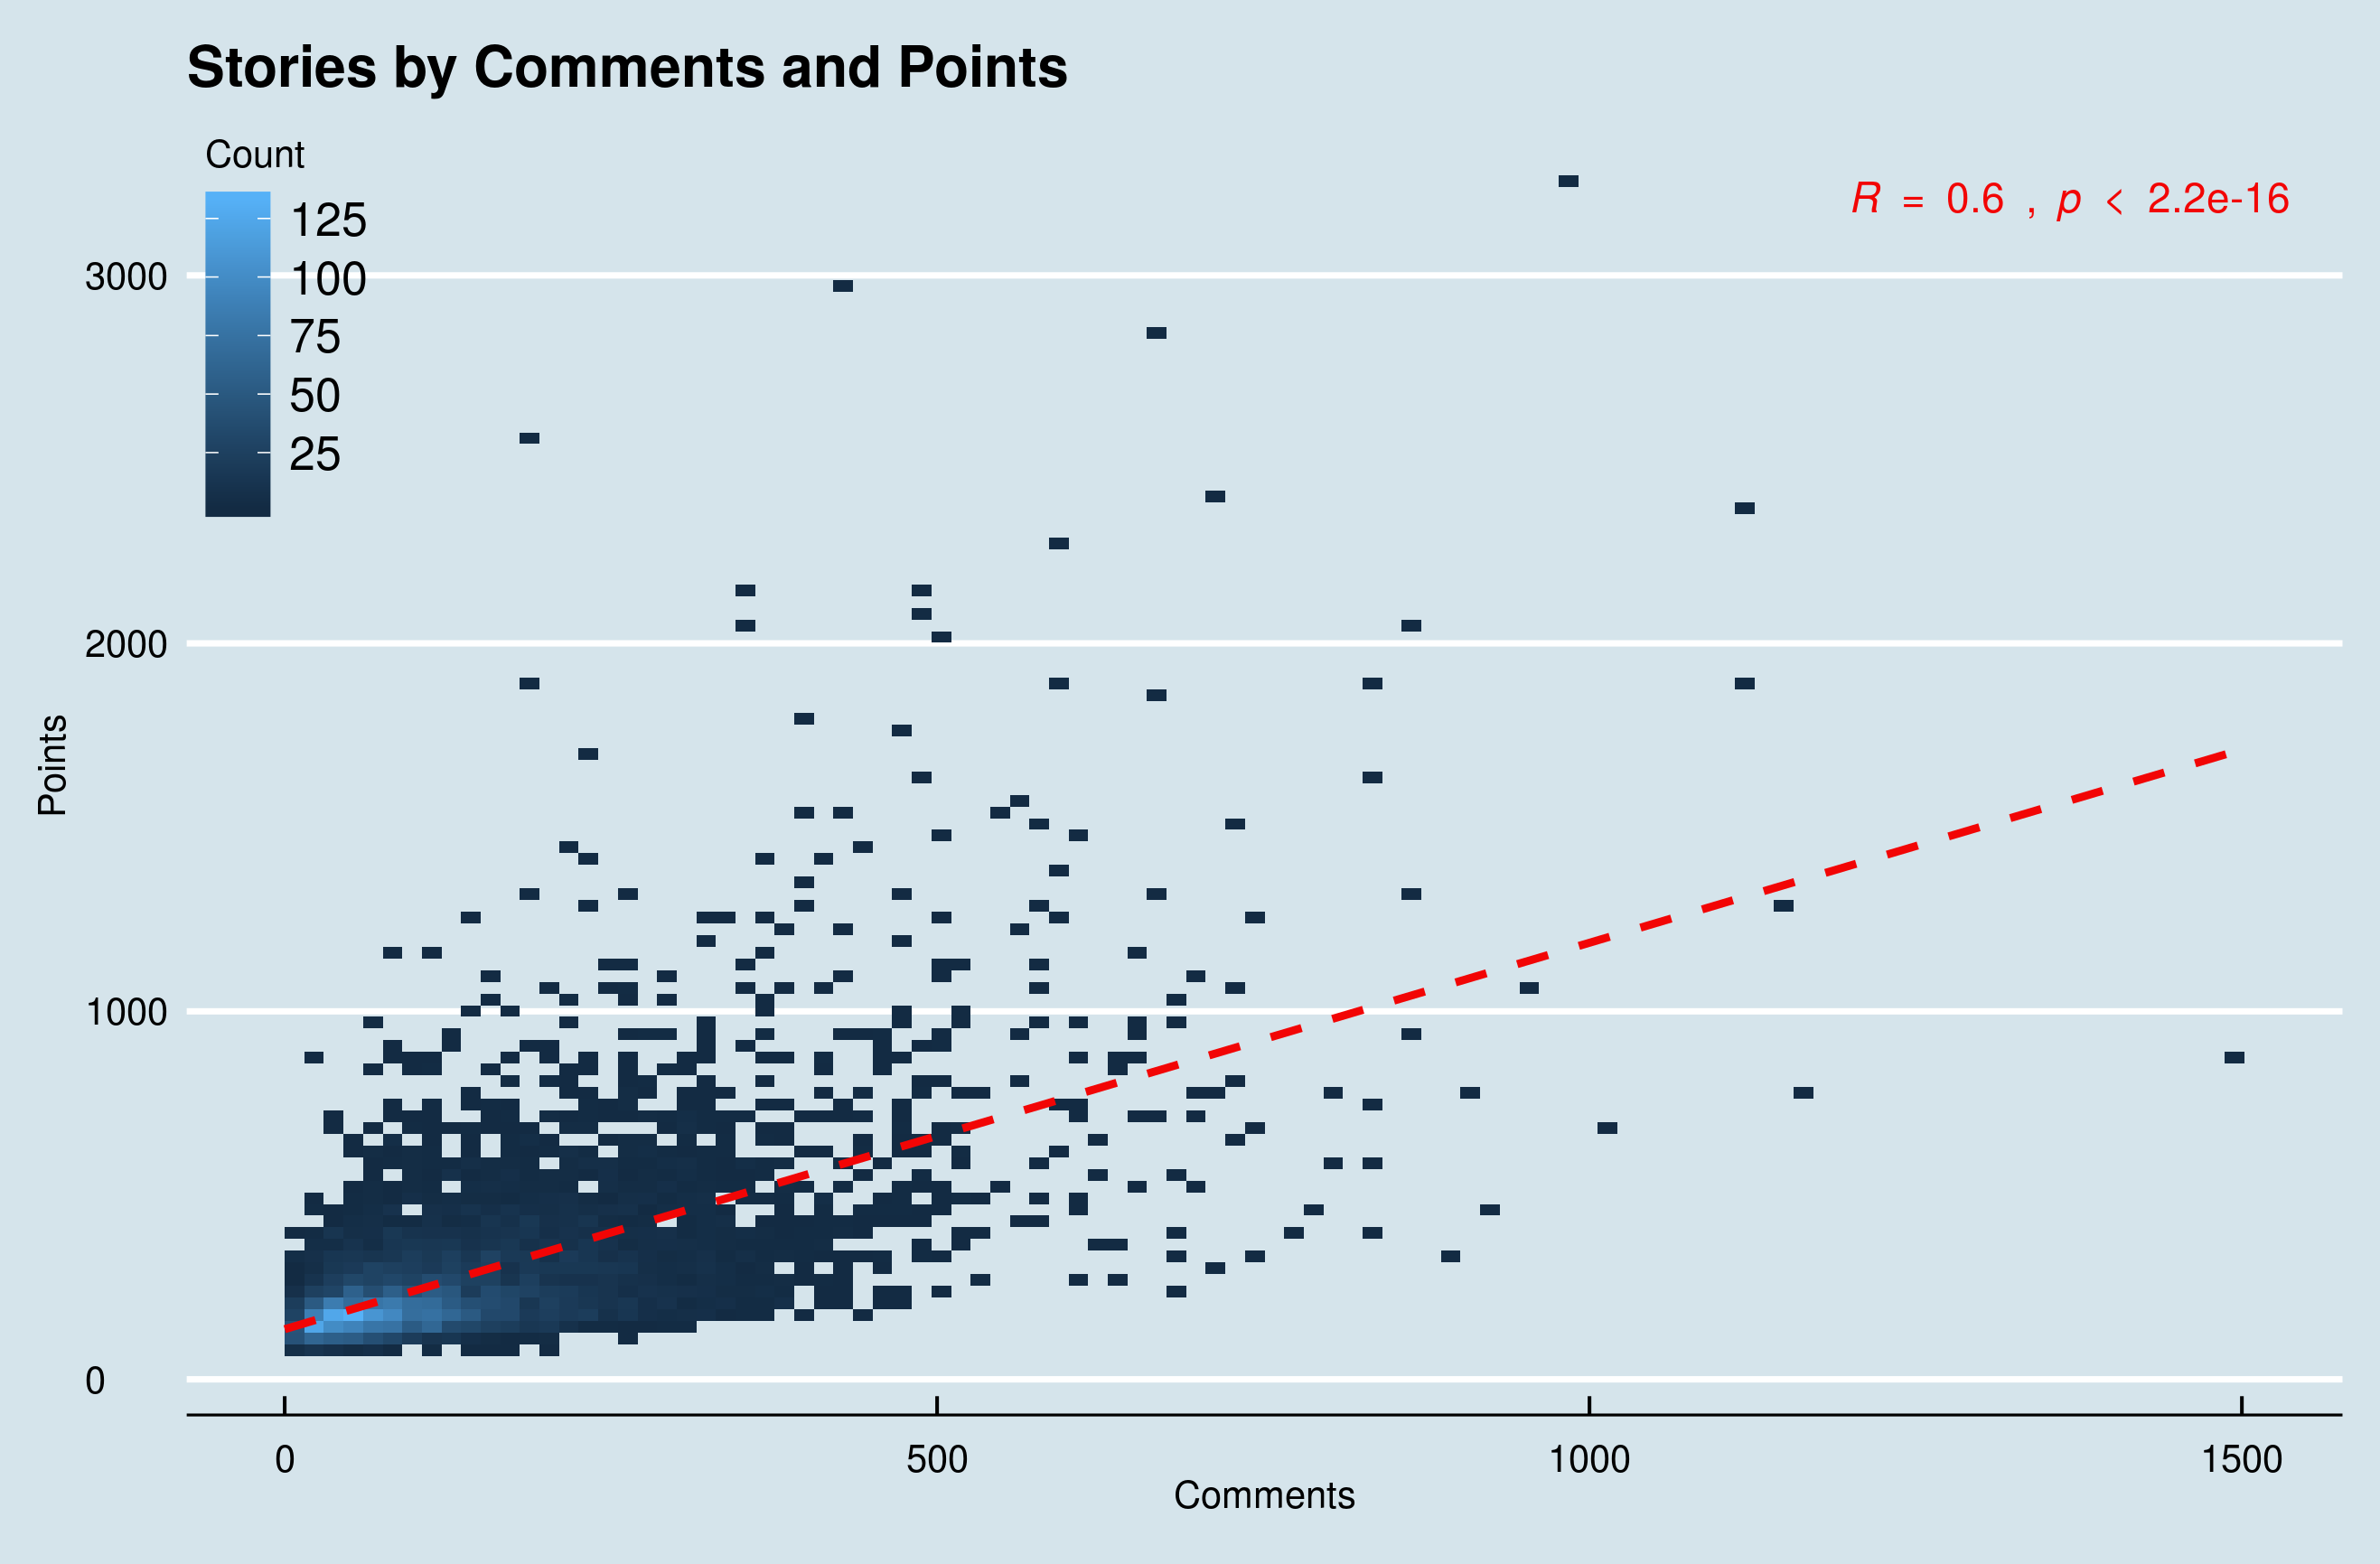
\includegraphics[scale=0.4]{img/descriptive_01_sources_bin.png}}
\caption{Stories plotted by Comments and Points within density bins}
\label{fig1}
\end{figure}

Perhaps unsurprisingly, we find that the relationship between the number of points assigned to an article, and the number of comments of an article is moderately correlated with a Pearson's R of 0.6 \cite{test:pearson}. 

The plot is gently skewed towards two directions - higher rated posts tend to receive fewer comments, while highly commented posts tend to receive less points. While strongly correlated, we observe that the regression line may not be as steep as expected because not every user who assigns an up-vote may comment and not every user who comments may assign an up-vote. 

\begin{figure}[!ht]
\centerline{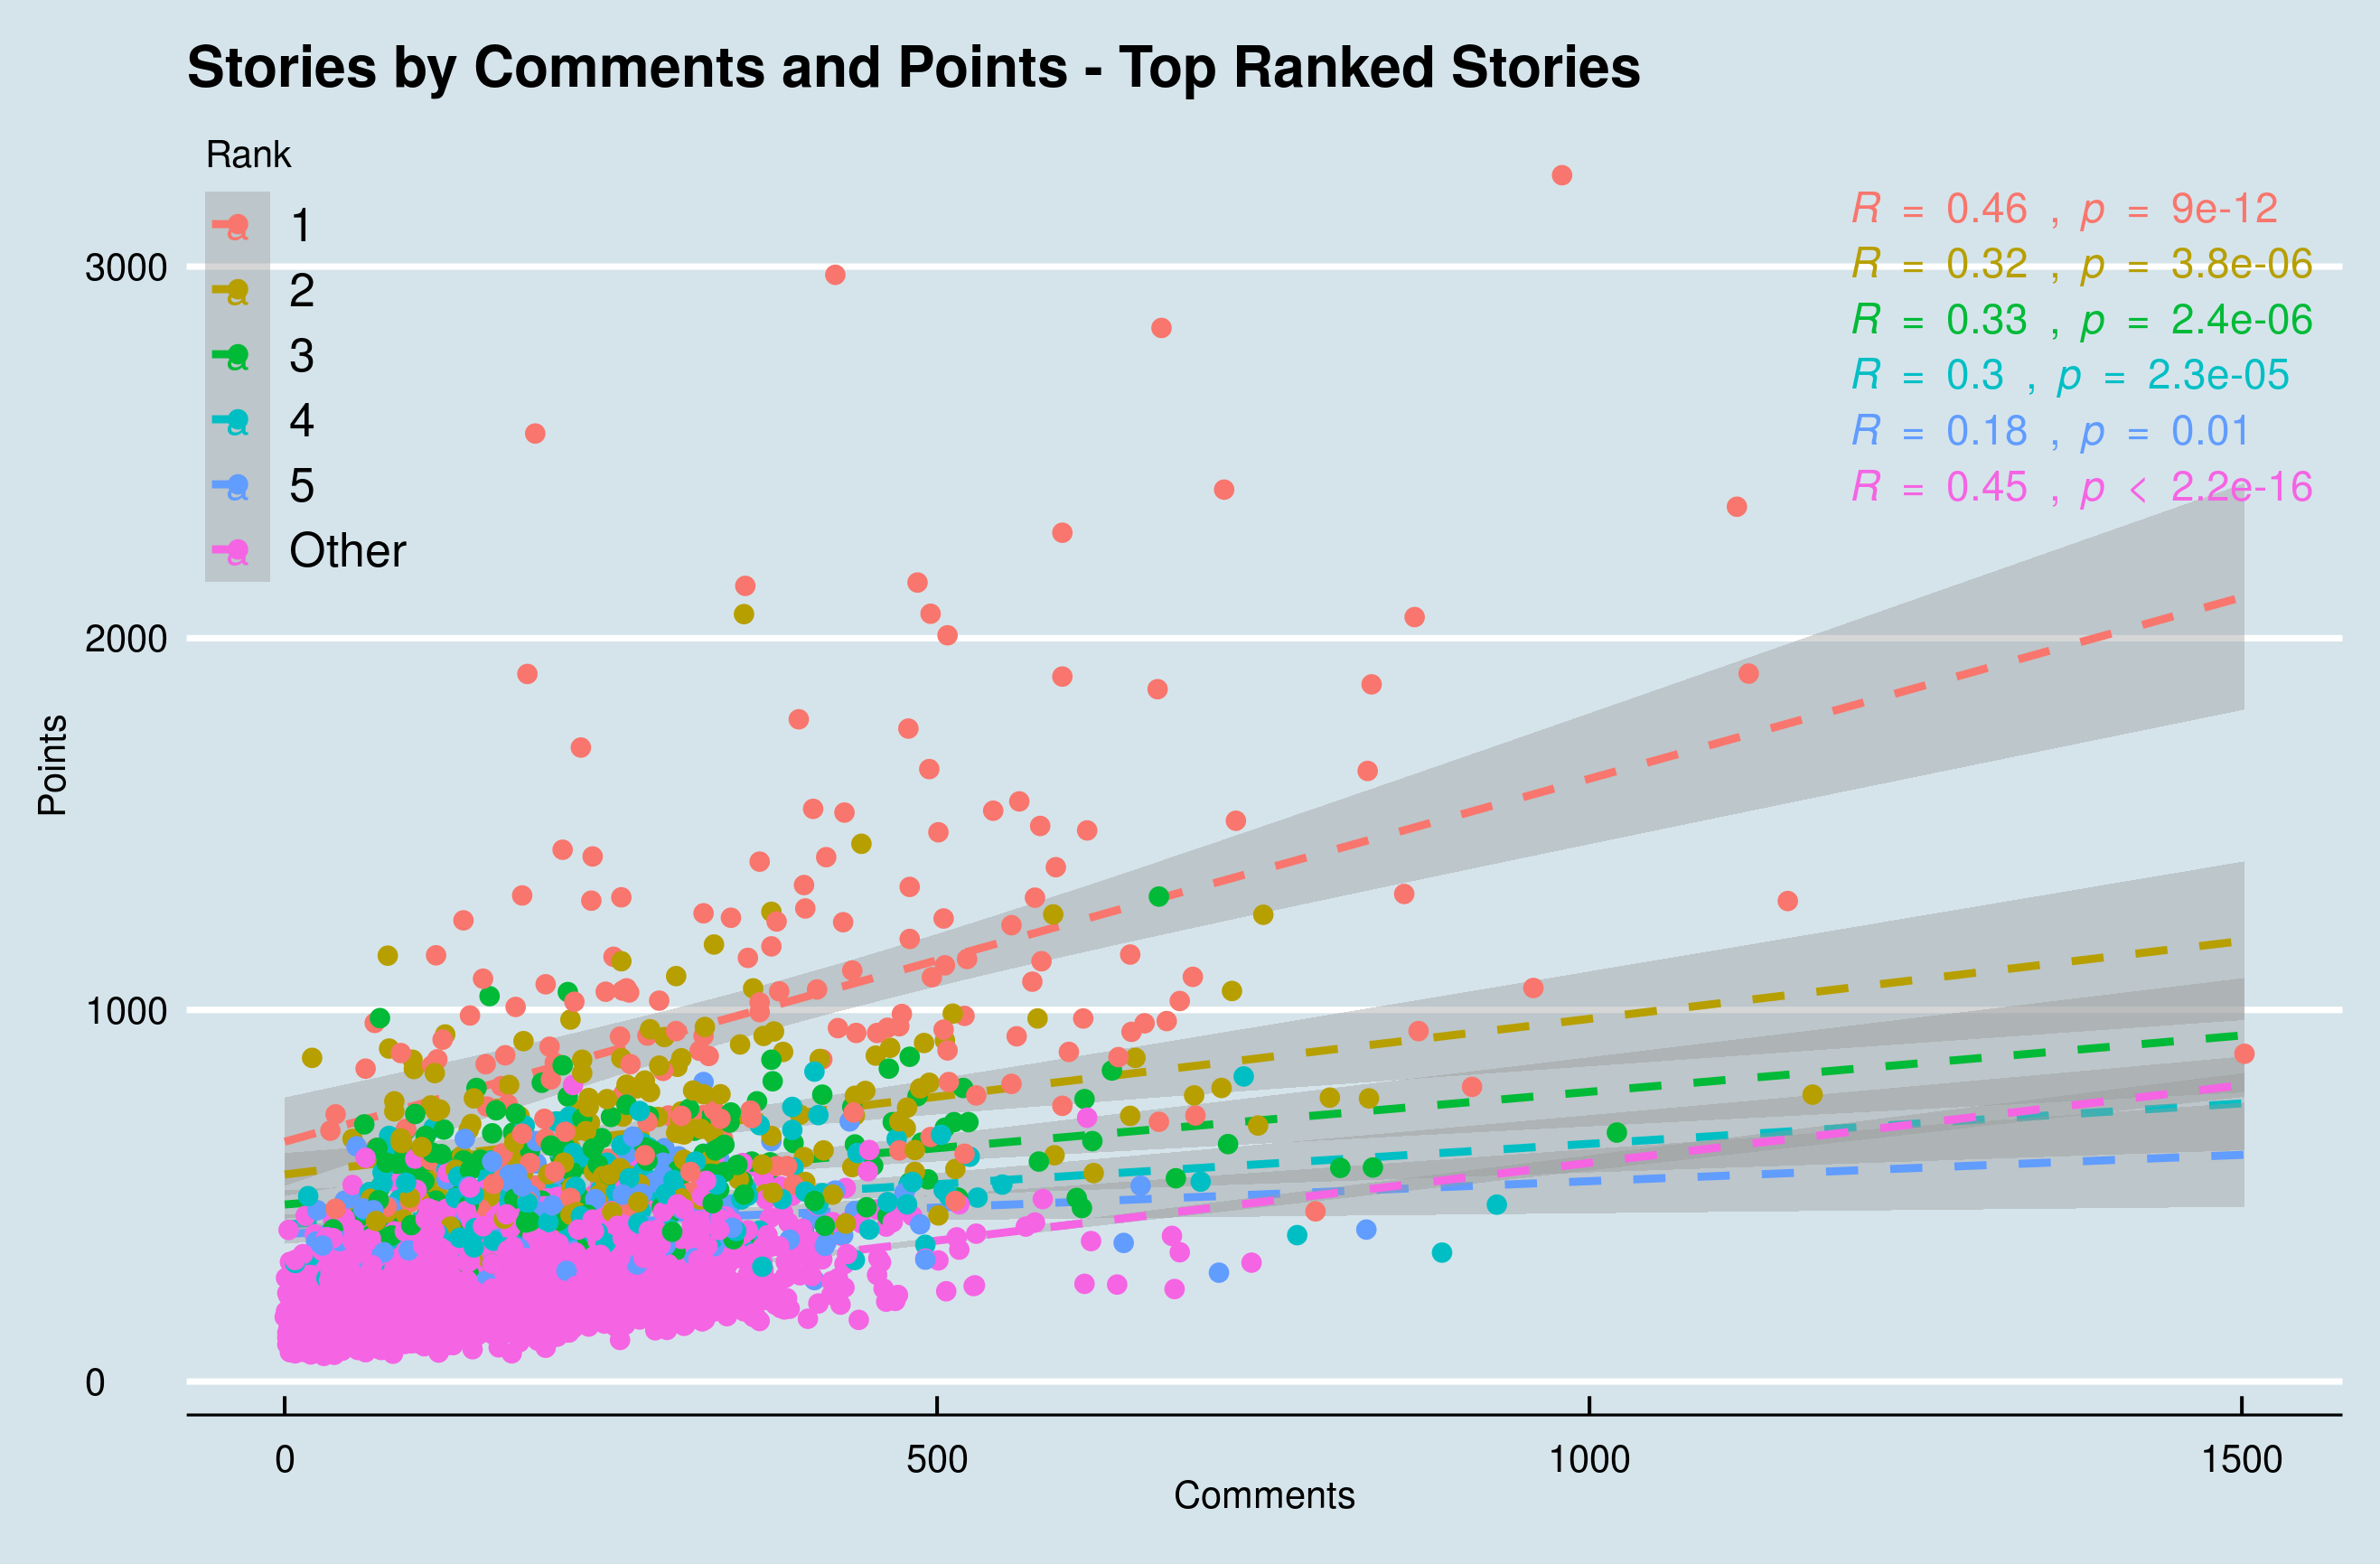
\includegraphics[scale=0.4]{img/descriptive_02_sources_rank.png}}
\caption{Stories plotted by Comments and Points grouped by Ranking}
\label{fig2}
\end{figure}

Laying motive for answering our second question regarding over-representation within the top post, we observe that articles with lower points tend to receive more comments than articles with higher points. 

To further illustrate this point, we plot the regression line for articles ranked within the top 5, and all other articles, showing a gentle reduction between point-comment correlation. In fact, for lower ranked articles, the correlation is weakly correlated. 

We also note that the correlation of the \textit{other} group is larger than that for articles ranked four and five, we attribute this to the size of the group. Given a plot which is further segmented, we would continue to see a reduction in the correlation until it flattens out.

Our observations are further corroborated by plotting the density curve for points and comments. Not only do stories tend to receive less comments than points, but we also observe that there is a larger variation in the number of comments an article receives, as opposed to the number of points. 

\begin{figure}[!ht]
\centerline{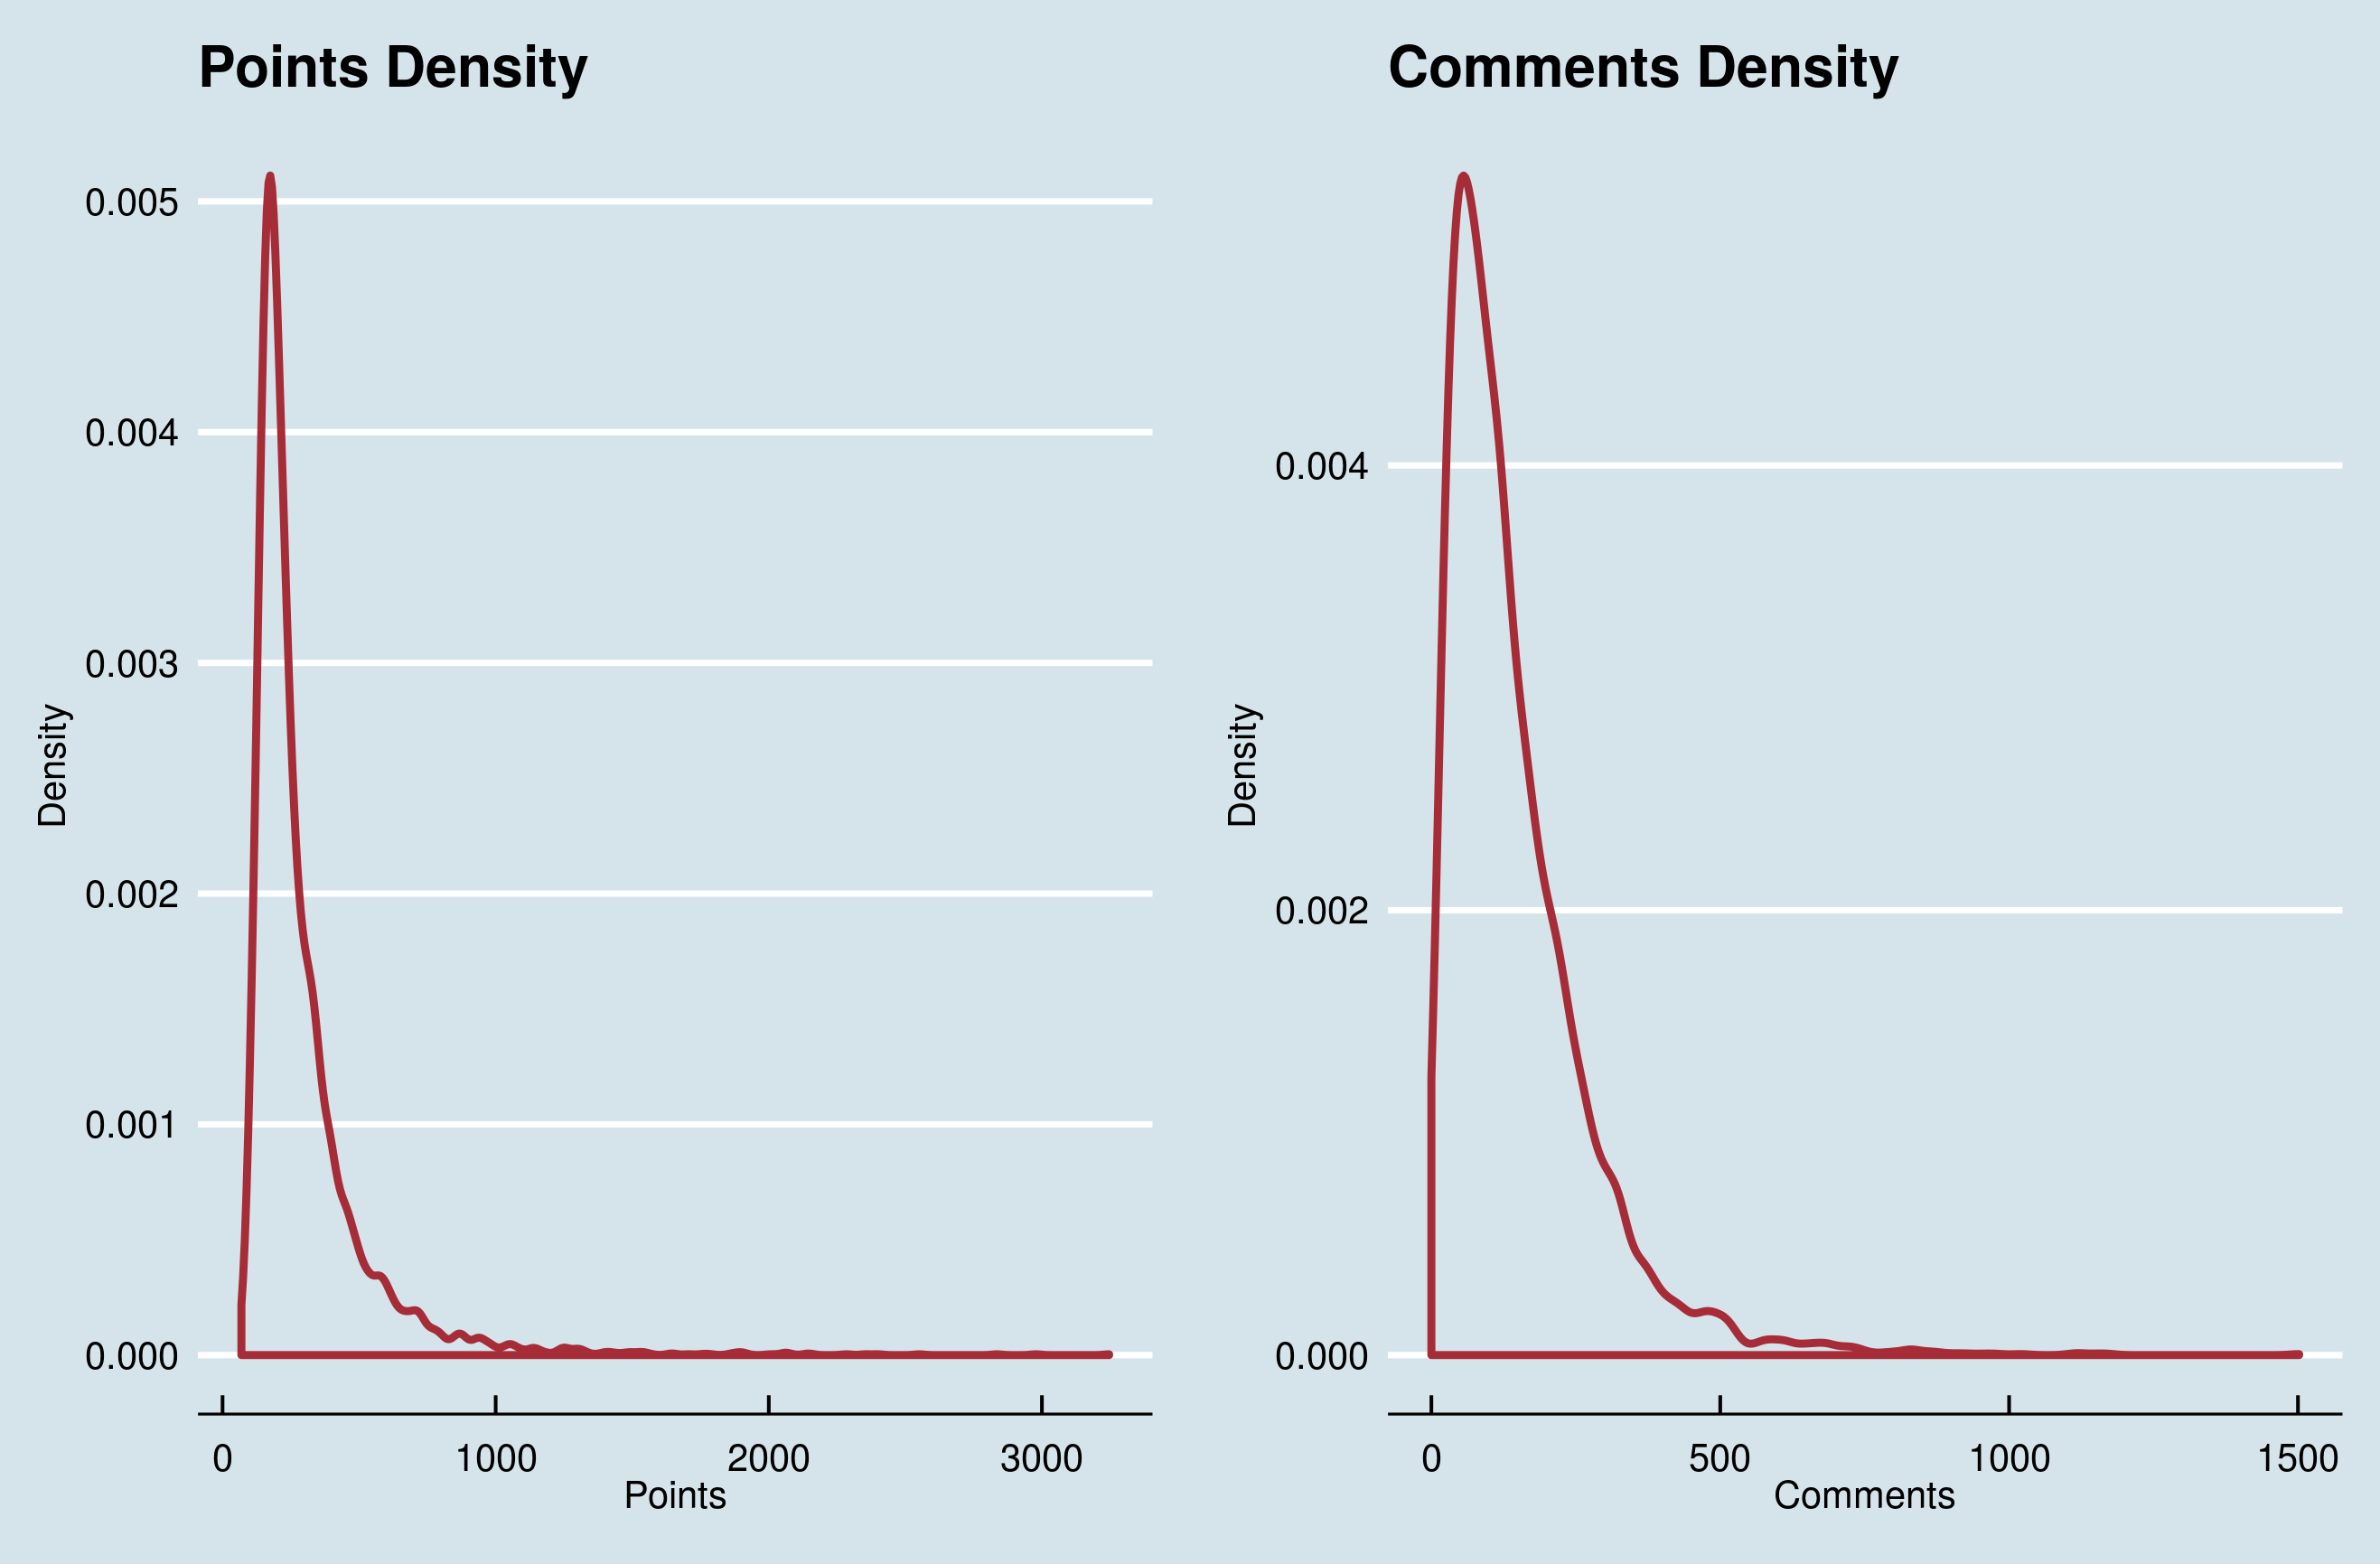
\includegraphics[scale=0.4]{img/descriptive_03_var_density.png}}
\caption{Density plot for points and comments}
\label{fig3}
\end{figure}

We extend our analysis of points and comments correlation to sources, noting that the correlation a strong correlation between points and comments for specific sources. The most widely commented and ranked sources are perhaps unsurprising, including popular news outlets such as the New York Times, Bloomberg, Techcrunch and social websites such as Github, Twitter and Medium. 
\begin{figure}[!ht]
\centerline{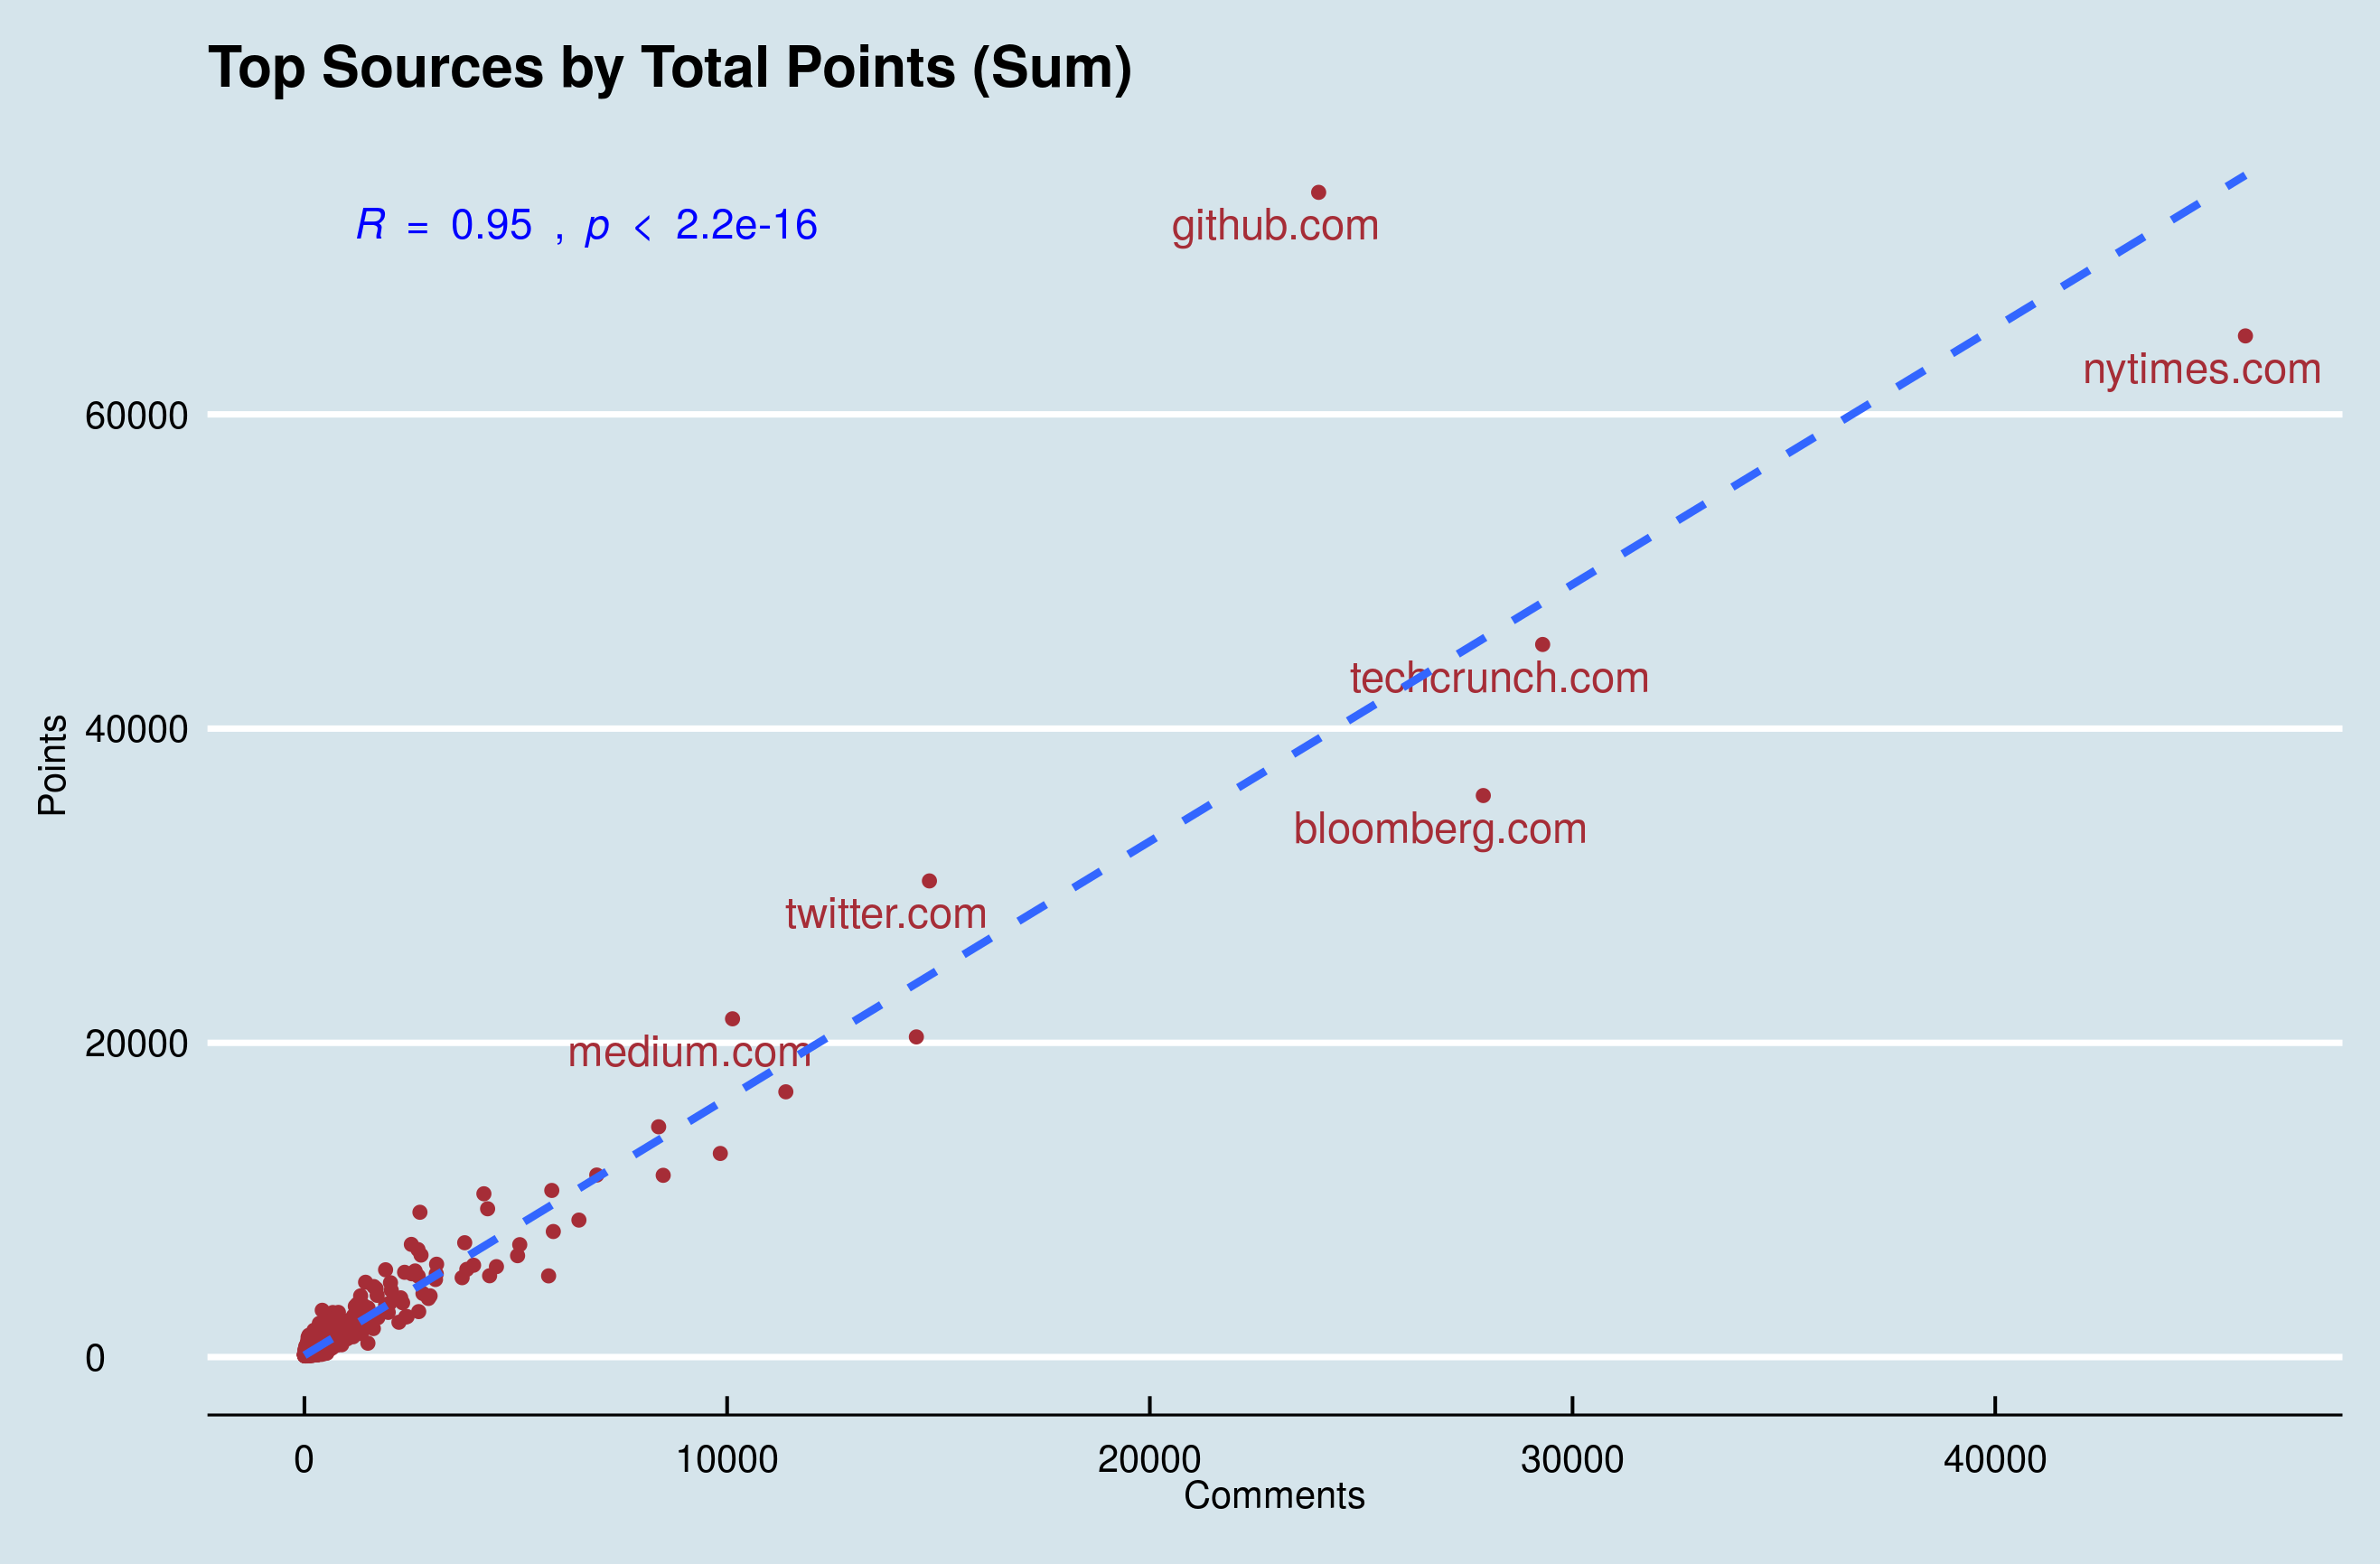
\includegraphics[scale=0.4]{img/descriptive_04_source_sum.png}}
\caption{Source Domains plotted by Sum of Comments and Points}
\label{fig4}
\end{figure}
We note that the correlation is clearer in this case primarily due to the fact that we are considering data sources which occur more frequently within the top hacker news rankings. A news outlet of the size and magnitude such as that of the New York Times, publishes more frequently than a lone developer's blog, thus it stands to reason that it ranks high within our analysis. 

However, the same plot for the \textit{median} number of points gives a very different picture. This plot is more representative of what can be considered to be quality Hacker News data sources, since it is not skewed by the frequency of stories. In fact, the correlation is similar to that presented in Figure 1.
\begin{figure}[!ht]
\centerline{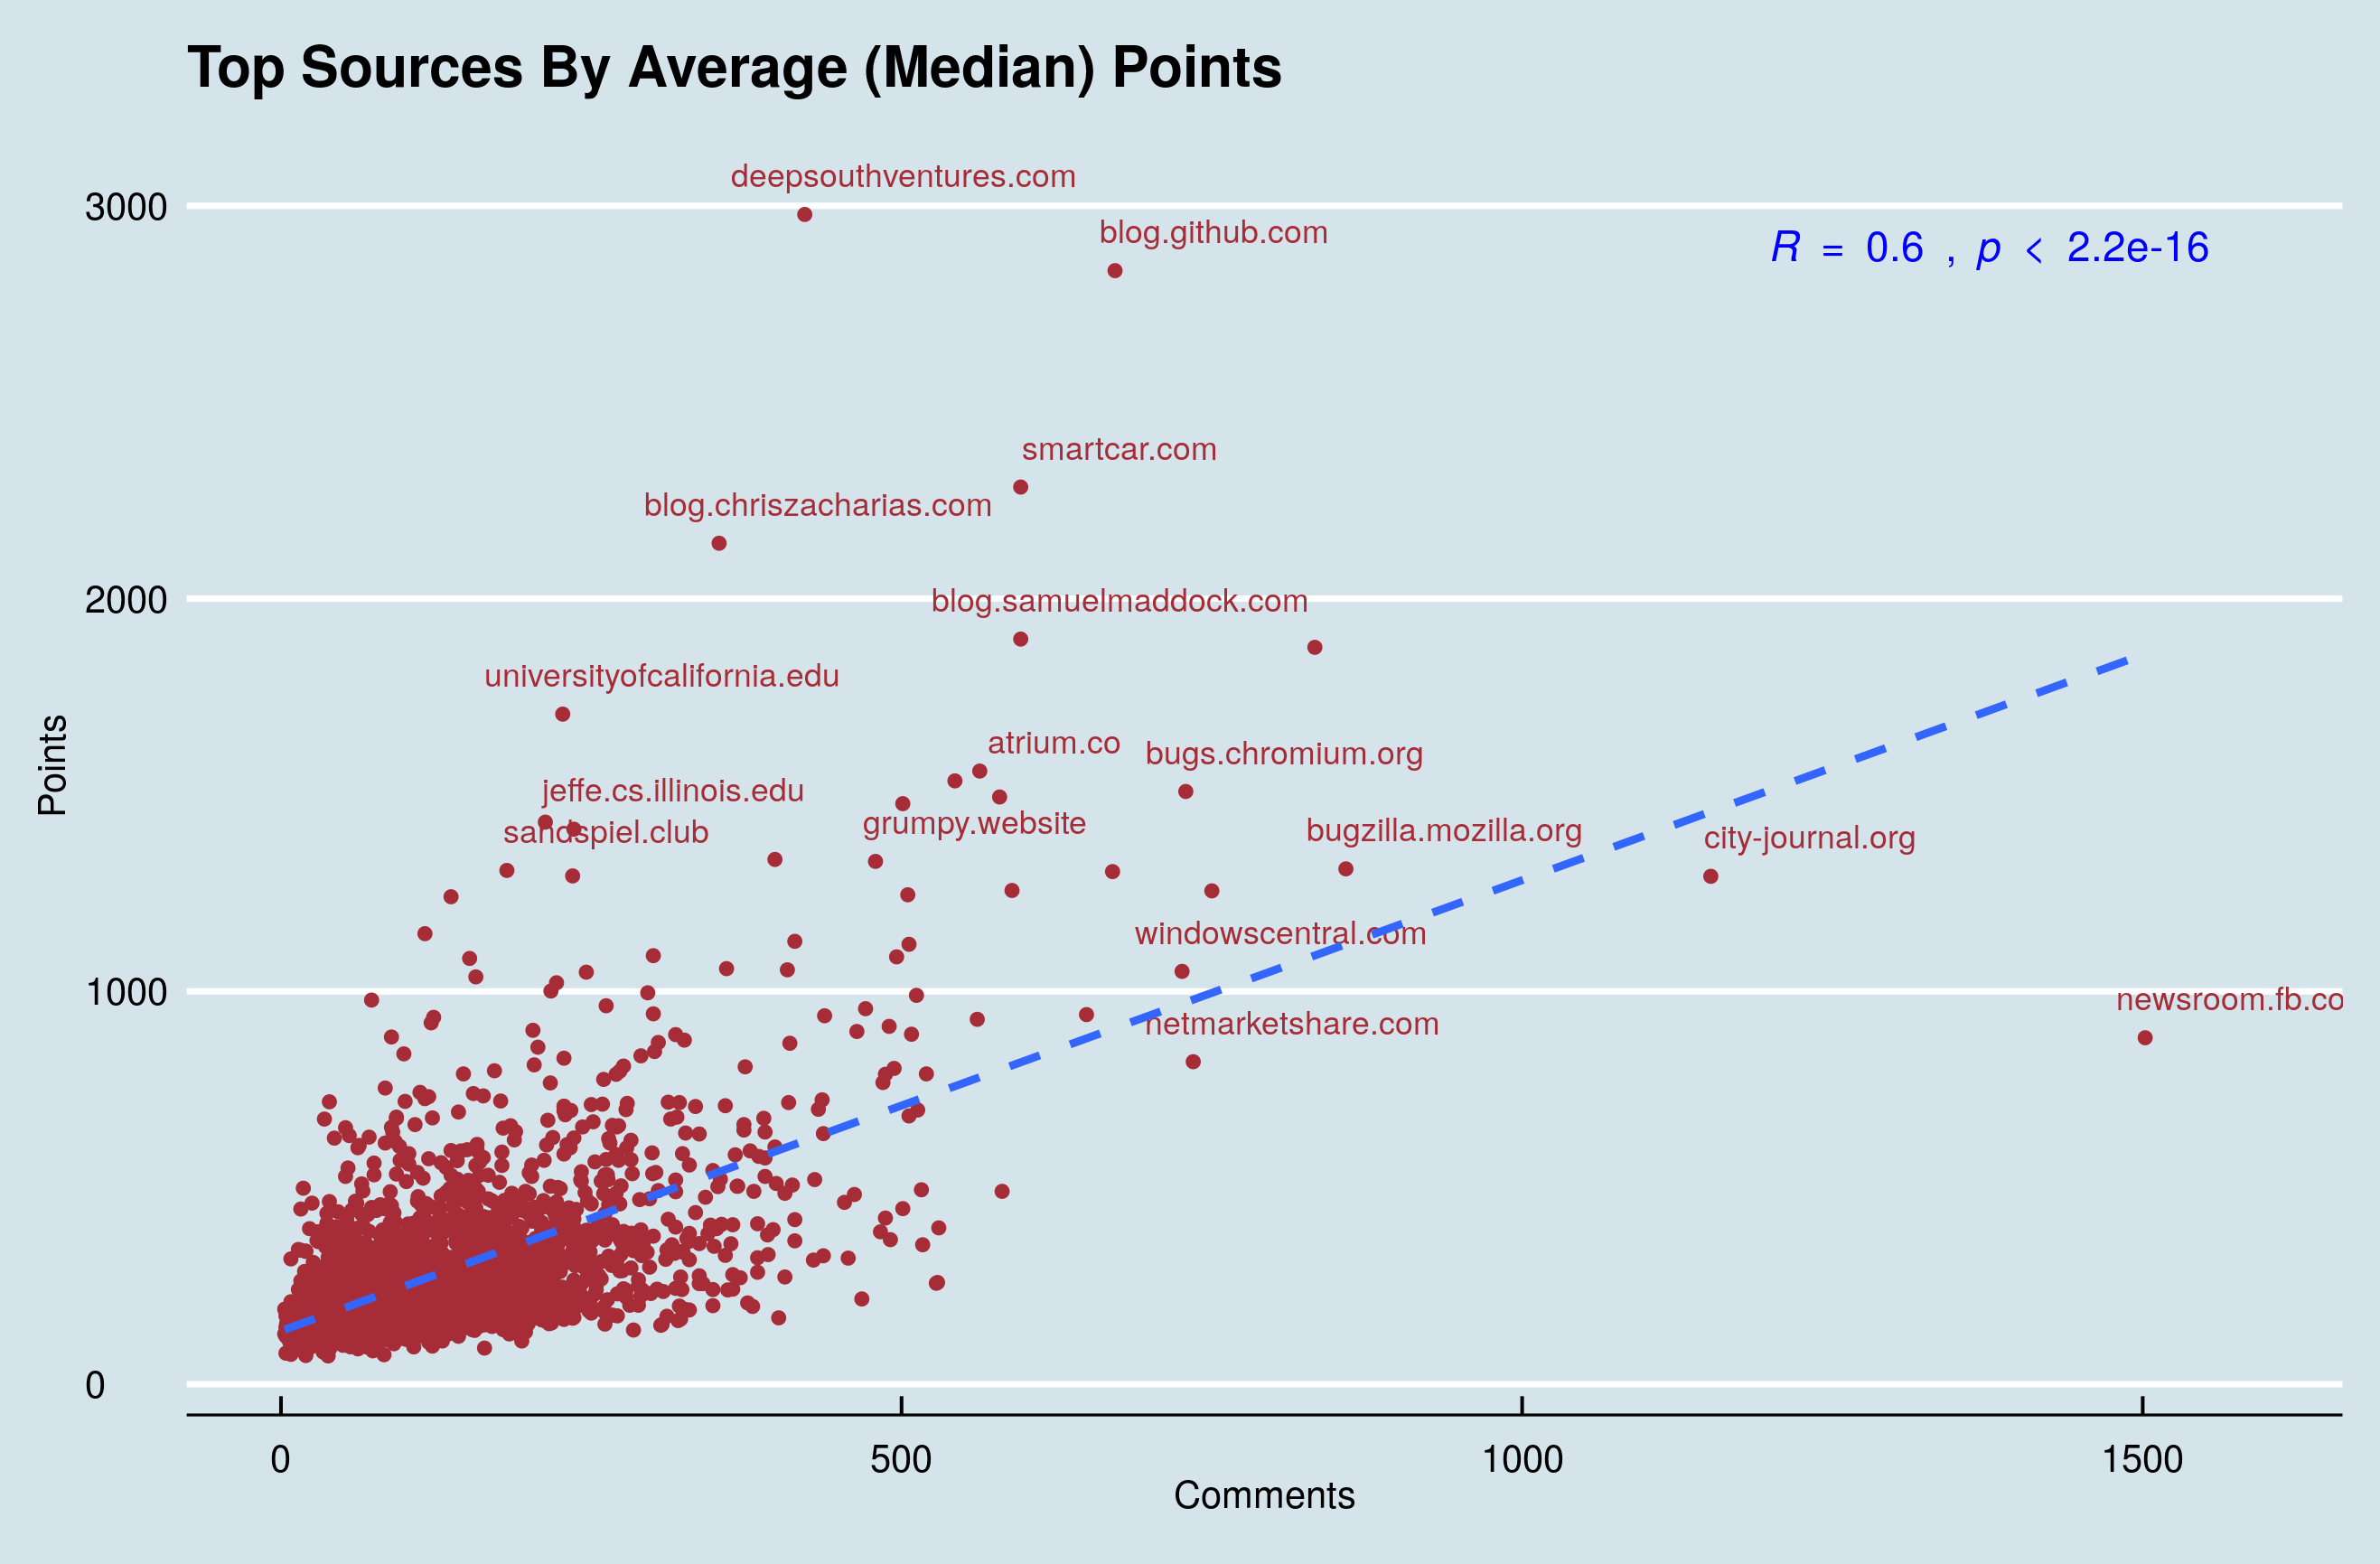
\includegraphics[scale=0.4]{img/descriptive_05_source_med.png}}
\caption{Source Domains plotted by Median of Comments and Points}
\label{fig5}
\end{figure}
In this plot, we may observe data sources with very few stories published to the board, which have been a major success serving as \textit{one hit wonders} of sorts. While GitHub retains its status as a top quality source on hacker news, the top voted source within our dataset is \textit{deepsouthventures.com} which has a very successful story related to bootstrapping an Onion sales startup. Similarly, it is followed by \textit{smartcar.com}, a startup whose product was cloned by a heavily funded competitor. 

Given the variety of data sources, we can qualitatively conclude that Hacker News serves its mission in providing articles which stimulate curiosity over simple corporate content.

We can conclude that content rules over quantity and power of association, however we also observe that the time of day is also indicative of the number of points a story receives. 
\begin{figure}[!ht]
\centerline{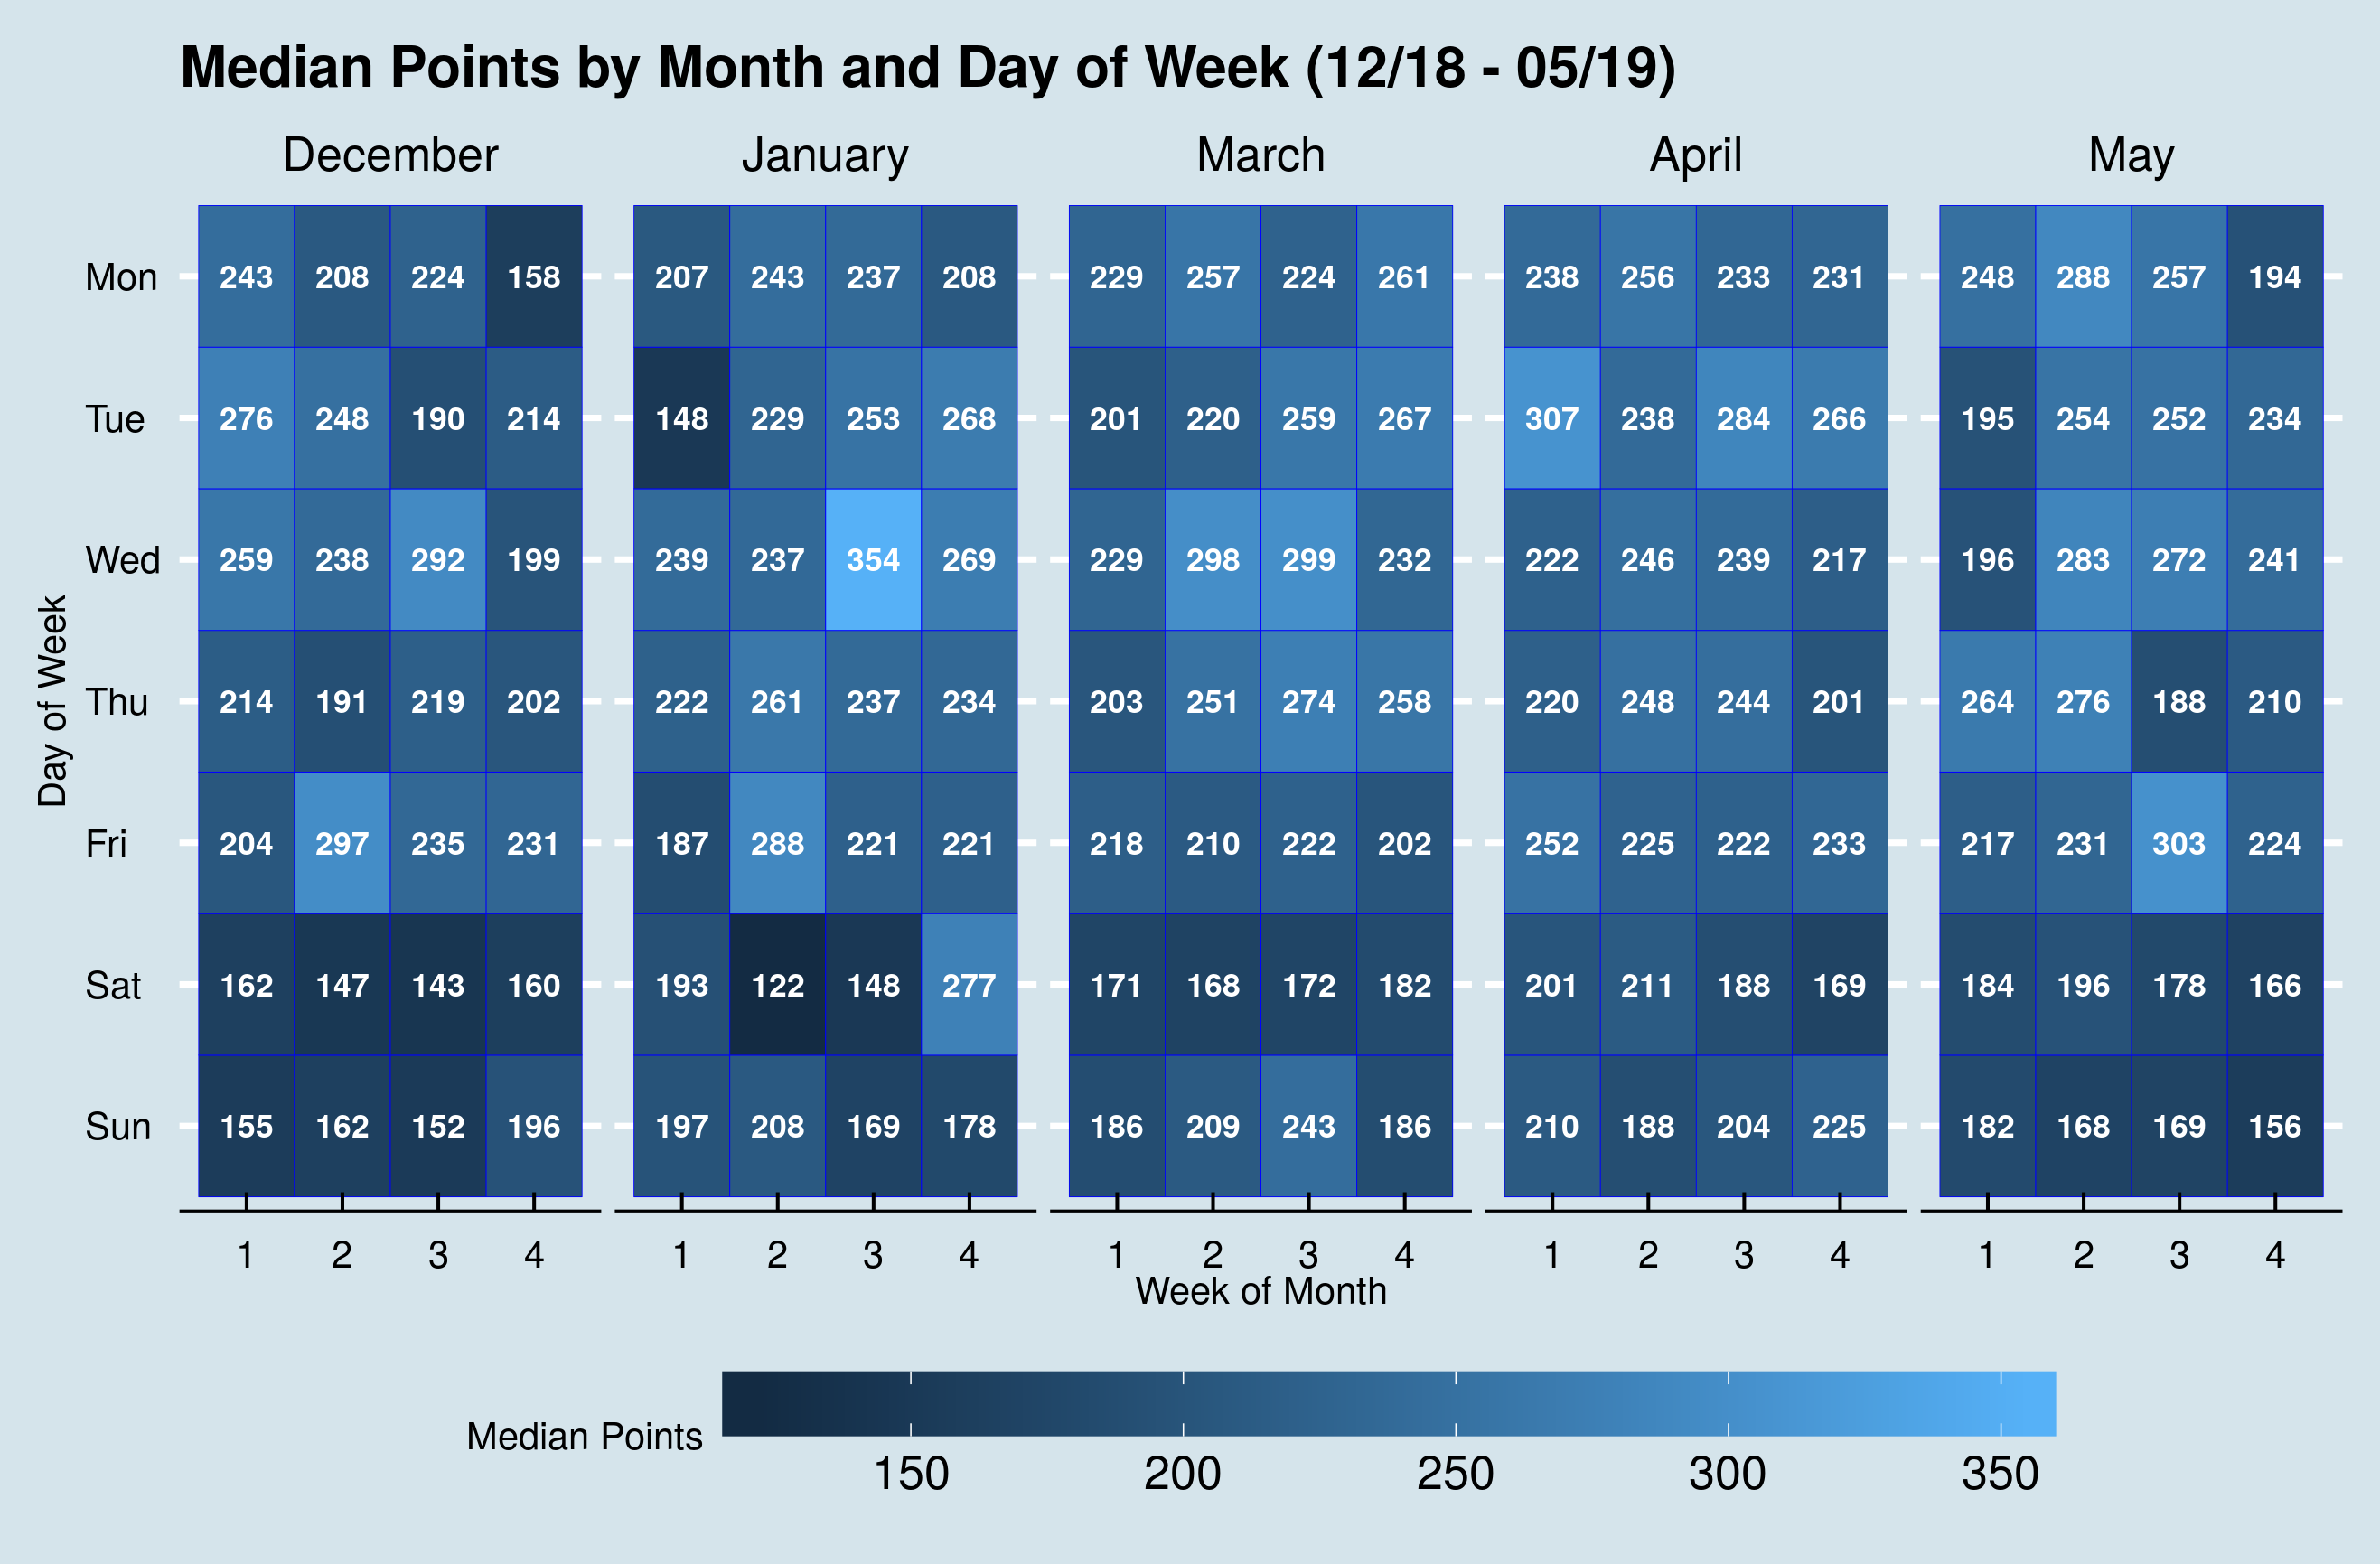
\includegraphics[scale=0.4]{img/descriptive_06_dayofweek.png}}
\caption{Heat-map of the median number of HN points by Month and Day of the Week}
\label{fig6}
\end{figure}

Next, we analyze stories based on the date and time being published. We note that a story may note necessarily be up-voted at the time of publishing, however stories do need to receive a number of up-votes in order to maintain their status on the front page; subsequently, the points on a story tend to compound as the hours pass. Thus, analyzing the date and time is necessary to understanding what constitutes a top post. 

\begin{figure}[!ht]
\centerline{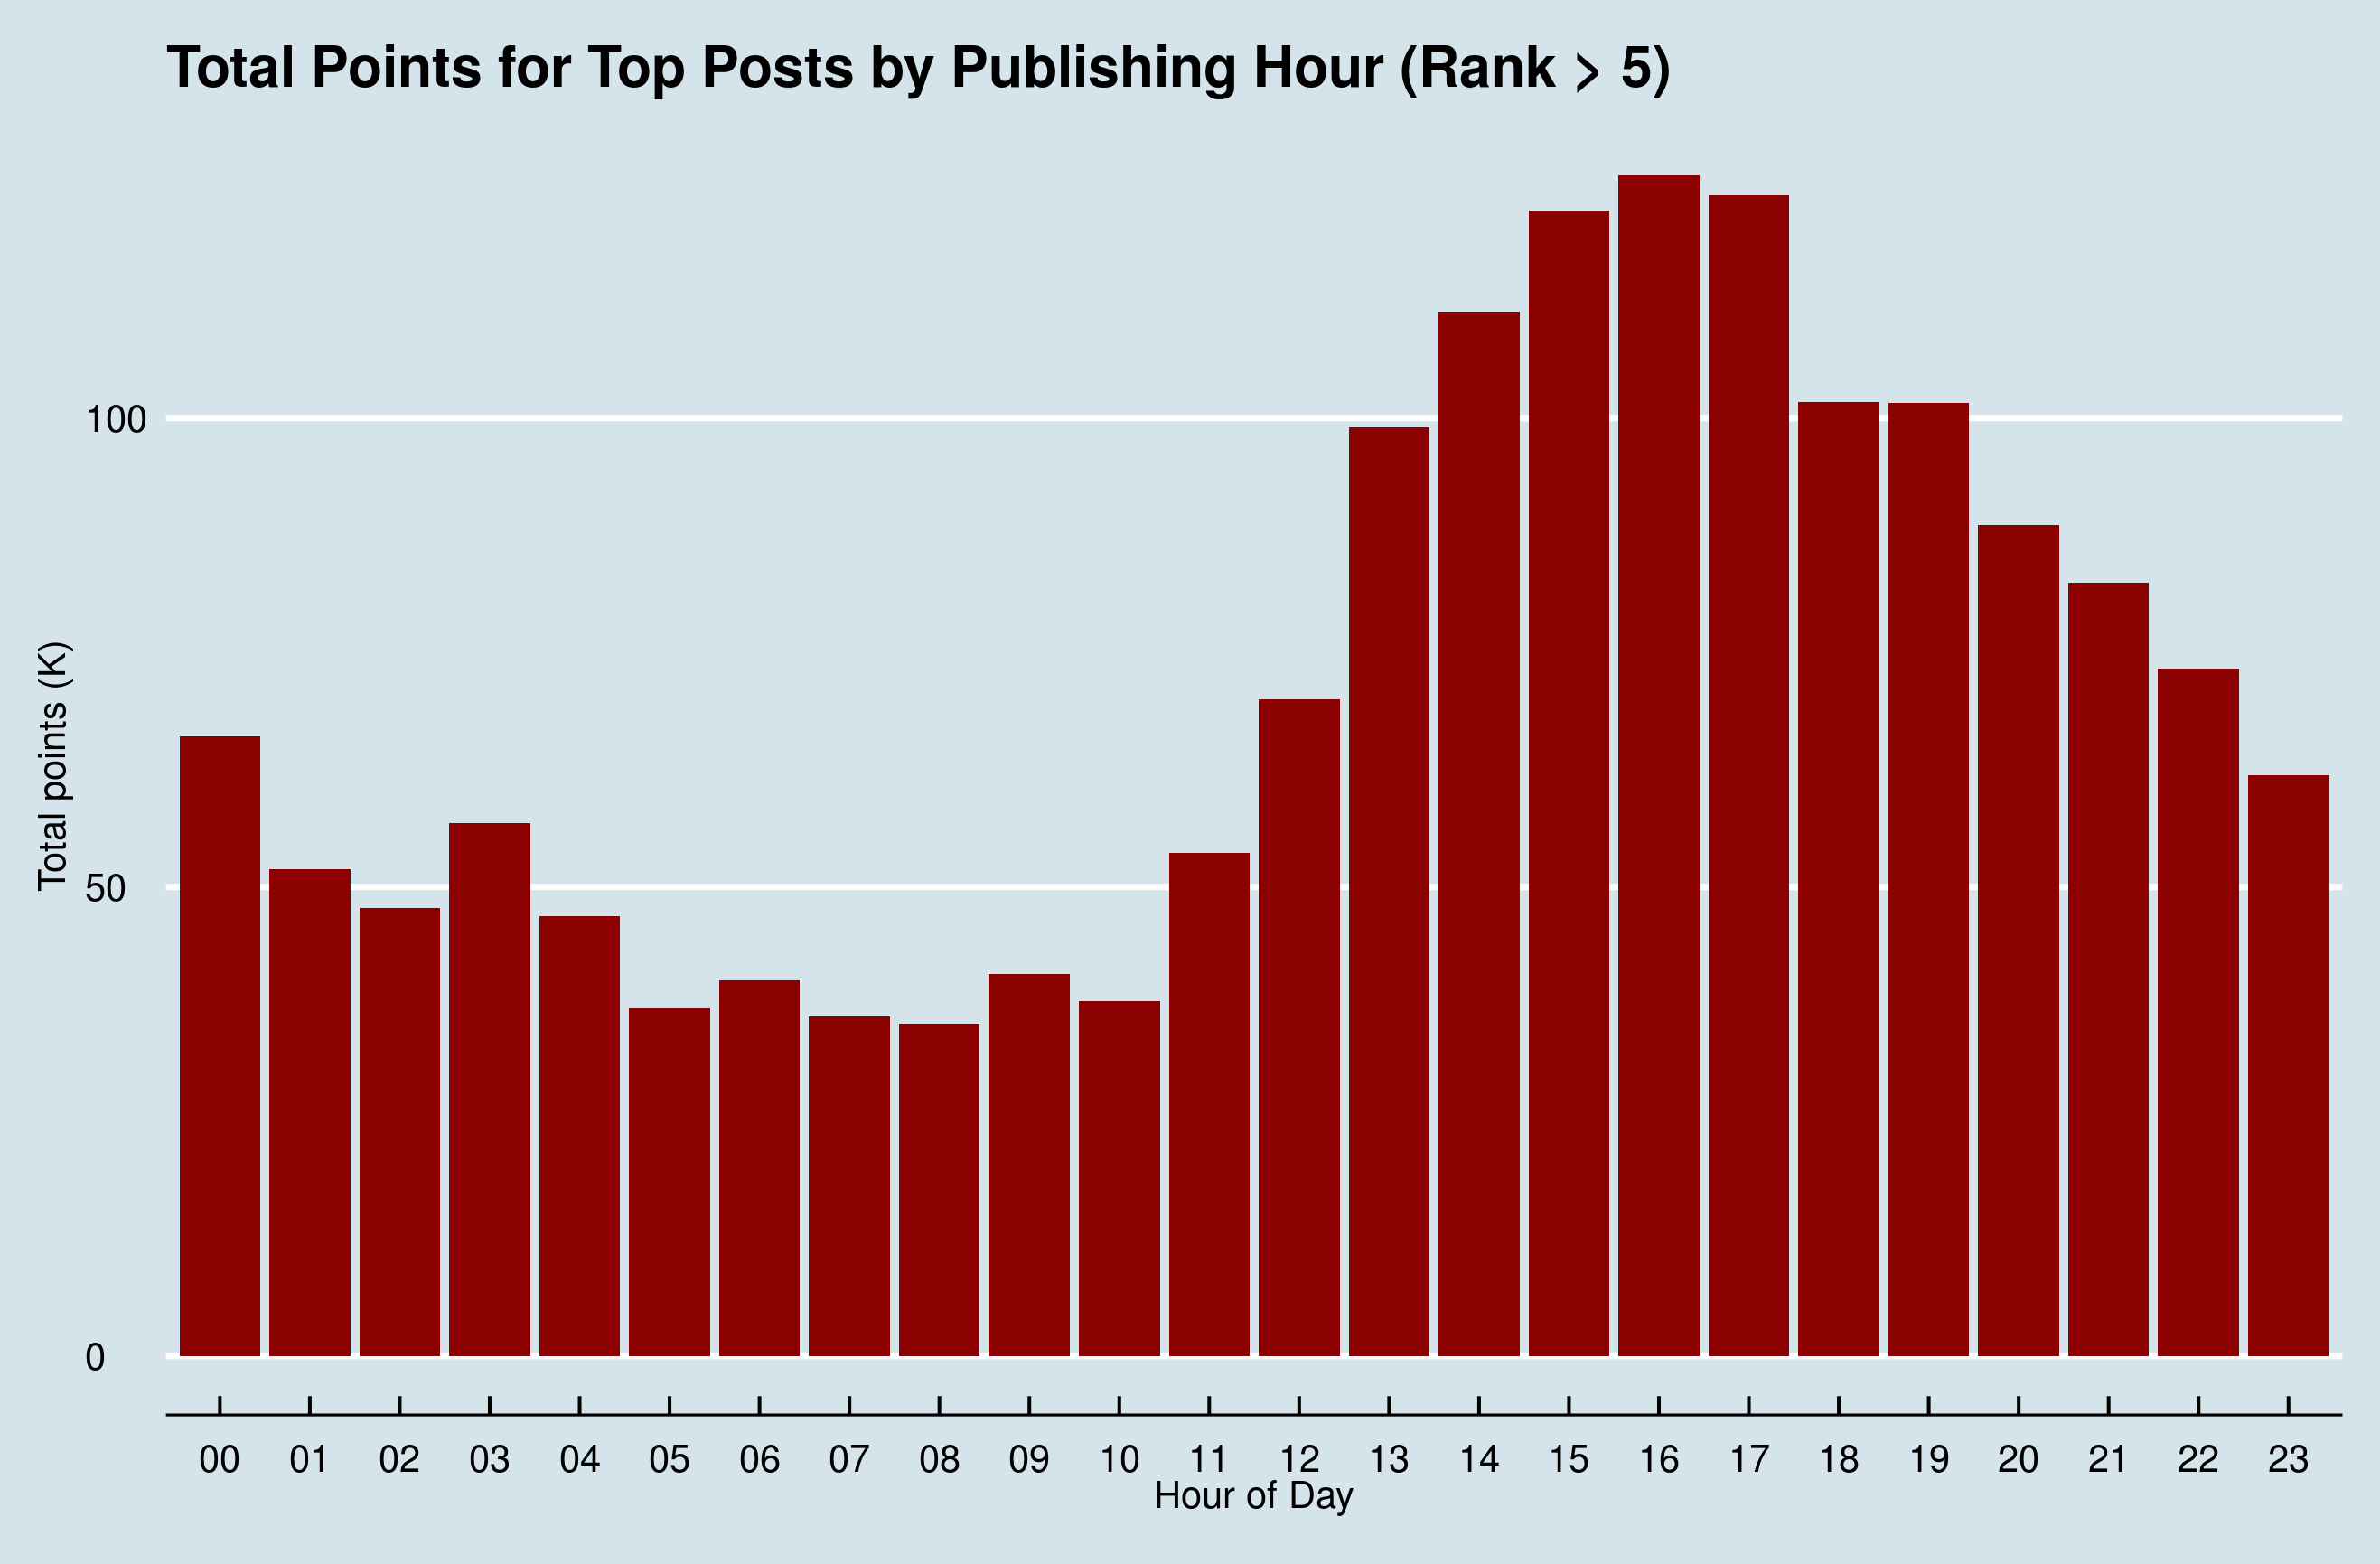
\includegraphics[scale=0.4]{img/descriptive_07_pointsbyhour.png}}
\caption{Points by Hour}
\label{fig7}
\end{figure}


The heat-map shows that HN articles published on weekdays are more successful than stories published on weekends. This can be attributed to the fact that since it is a data source which caters for business-related news, users frequent the site more often during business hours. Alternatively, one can hypothesize that HN is considered to be a healthier workplace distraction than other social media websites, however this hypothesis is difficult to substantiate.

To investigate this phenomenon, we investigate the number of points by the hour of the day. A visual inspection of the histogram of points shows that articles published later on in the day tend to be more successful than those published in the morning. Stories published between 2pm and 7pm tend to receive the most points.

The top posted articles tend to be posted after lunch time or during the night, possibly indicating that HN does indeed serve as a distraction, either from the workplace or from the bedtime. Finally, we extract a word cloud of terms from the story headlines, giving us an indication of what topics to expect within the topic analysis section; in particular, it drives our decision to limit our topic detection to texts containing noun phrases and verb phrases.

\section{Topic Detection}
We train our LDA model using 5,939 documents containing 7,947 terms, observing that the dataset is highly sparse.  

\begin{table}[!ht]
\centering
\begin{tabular}{ll}
\hline
\multicolumn{2}{l}{Document Term Matrix} \\ \hline
Documents             & 5,939            \\ \hline
Terms                 & 7,947            \\ \hline
Sparsity              & 99\%             \\ \hline
\\
\end{tabular}
\caption{Document Term Matrix for LDA Training}
\label{tab:dtmatrix}
\end{table}

Next, we perform the \textit{parameter selection process} by repeatedly running the model for $K$ values one through 120, at 700 iterations with a burn-in rate of 200. After each run, we calculate the Maximum Log-Likelihood (LL) of the model to evaluate the topic mixture. We cease our testing when the Maximum LL begins to taper off, seemingly converging. Figure \ref{fig7} shows the Maximum LL plotted against $K$, showing the ideal $K$ to be 114 topics.

\begin{figure}[!ht]
\centerline{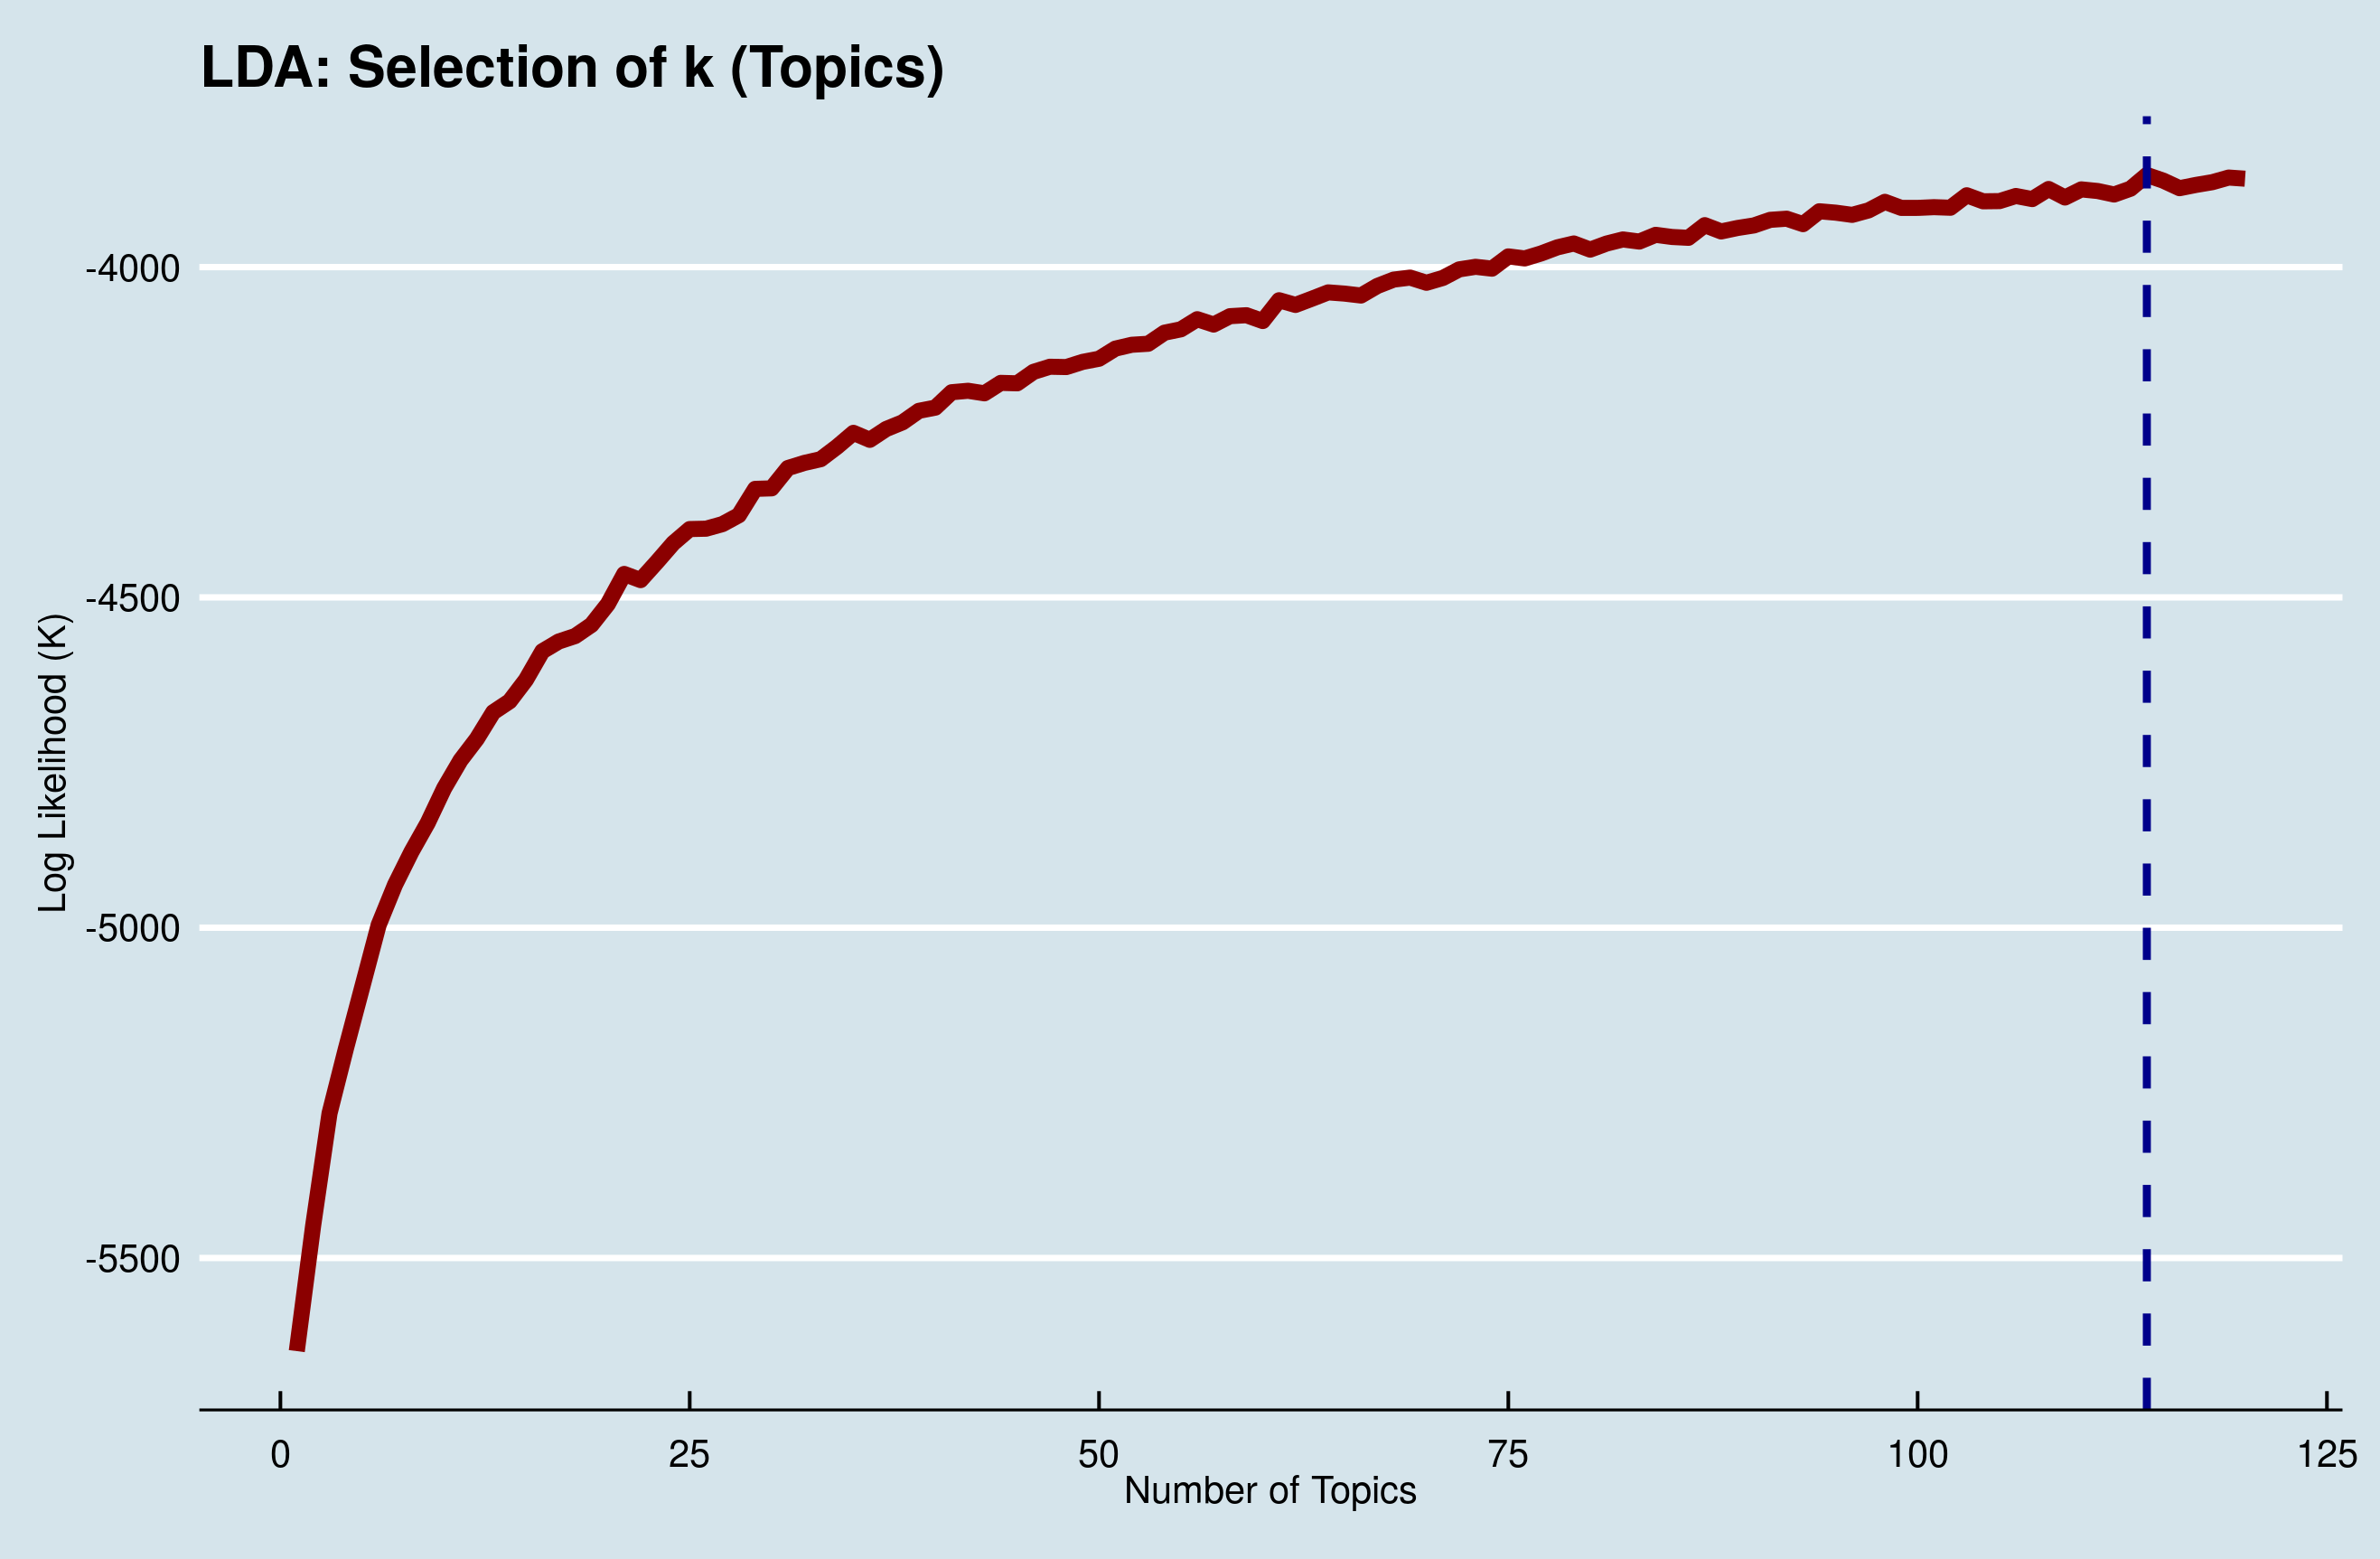
\includegraphics[scale=0.4]{img/topic_model_01_idealk.png}}
\caption{K Selection Process}
\label{fig7}
\end{figure}

The LDA model outputs a series of topics, identified by their keywords. Each topic was evaluated, and annotated with a brief human-readable description in order to facilitate analysis. Table \ref{tab:annot-examples} shows a number of examples. Most of the topics are clearly discernable as pertaining to a particular topic, however 18 of the 114 topics were identified as \textit{noisy topics}, which did not have a single discernable topic.

\begin{table}[!ht]
\centering
\tiny
\begin{tabular}{lll}
\hline
\begin{tabular}[c]{@{}l@{}}Topic\\ Id\end{tabular} & Keywords                            & \begin{tabular}[c]{@{}l@{}}Human-Readable\\ Annotation\end{tabular} \\ \hline
1                                                  & point view channel youtub content   & Youtube                                                             \\ \hline
2                                                  & flight plane air boe pilot          & Boeing 737 \& Aviation                                              \\ \hline
3                                                  & countri india germani europ world   & Geopolitics                                                         \\ \hline
4                                                  & phone devic call android smartphon  & Mobile Devices \& Apps                                              \\ \hline
5                                                  & life friend mind world advic        & Self Improvement                                                    \\ \hline
6                                                  & rust webassembl red swift runtim    & Rust Lang.                                                          \\ \hline
7                                                  & materi glass plastic wast wood      & Environmental Concerns                                              \\ \hline
8                                                  & earth moon land planet star         & Space Exploration                                                   \\ \hline
9                                                  & compani fund investor capit founder & VC,IPOs \& Money                                                    \\ \hline
10                                                 & editor edit guid emac studio        & IDEs                                                                \\ \hline
11                                                 & money peopl dollar million thousand & Making Money                                                        \\ \hline
12                                                 & peopl decis lot problem fact        & Quitting Jobs \& Toxic SV Culture                                   \\ \hline
13                                                 & ’ ’ve lot ’ll note                  & Noisy Topic 1                                                       \\ \hline
14                                                 & perform intel cpu processor core    & CPUs, Performance \& Advances                                       \\ \hline
15                                                 & market busi industri compani sale   & Corporate Revenue \& Transactions                                   \\ \hline
\\
\end{tabular}
\caption{Examples of Human-Readable Annotations Assigned to LDA Topics}
\label{tab:annot-examples}
\end{table}

The topics detected span a wide range of subjects. Our qualitative annotation exercise reveals that Hacker News is a diverse bulletin board, referencing stories spanning from software development, consumer electronics, psychology, self-help, business and the environment. Some topics treat programming languages such as Rust and Ruby, while others deal with programming niches such as Numerical Computing, Machine Learning and Concurrency. Moreover, we observe a large number of topics relating to self-help, psychology, geo-politics and the environment.

Similar to our descriptive analysis, we plot topics by the median points and comments, showing us a visual indication of the most successful topics.

\begin{figure}[!ht]
\centerline{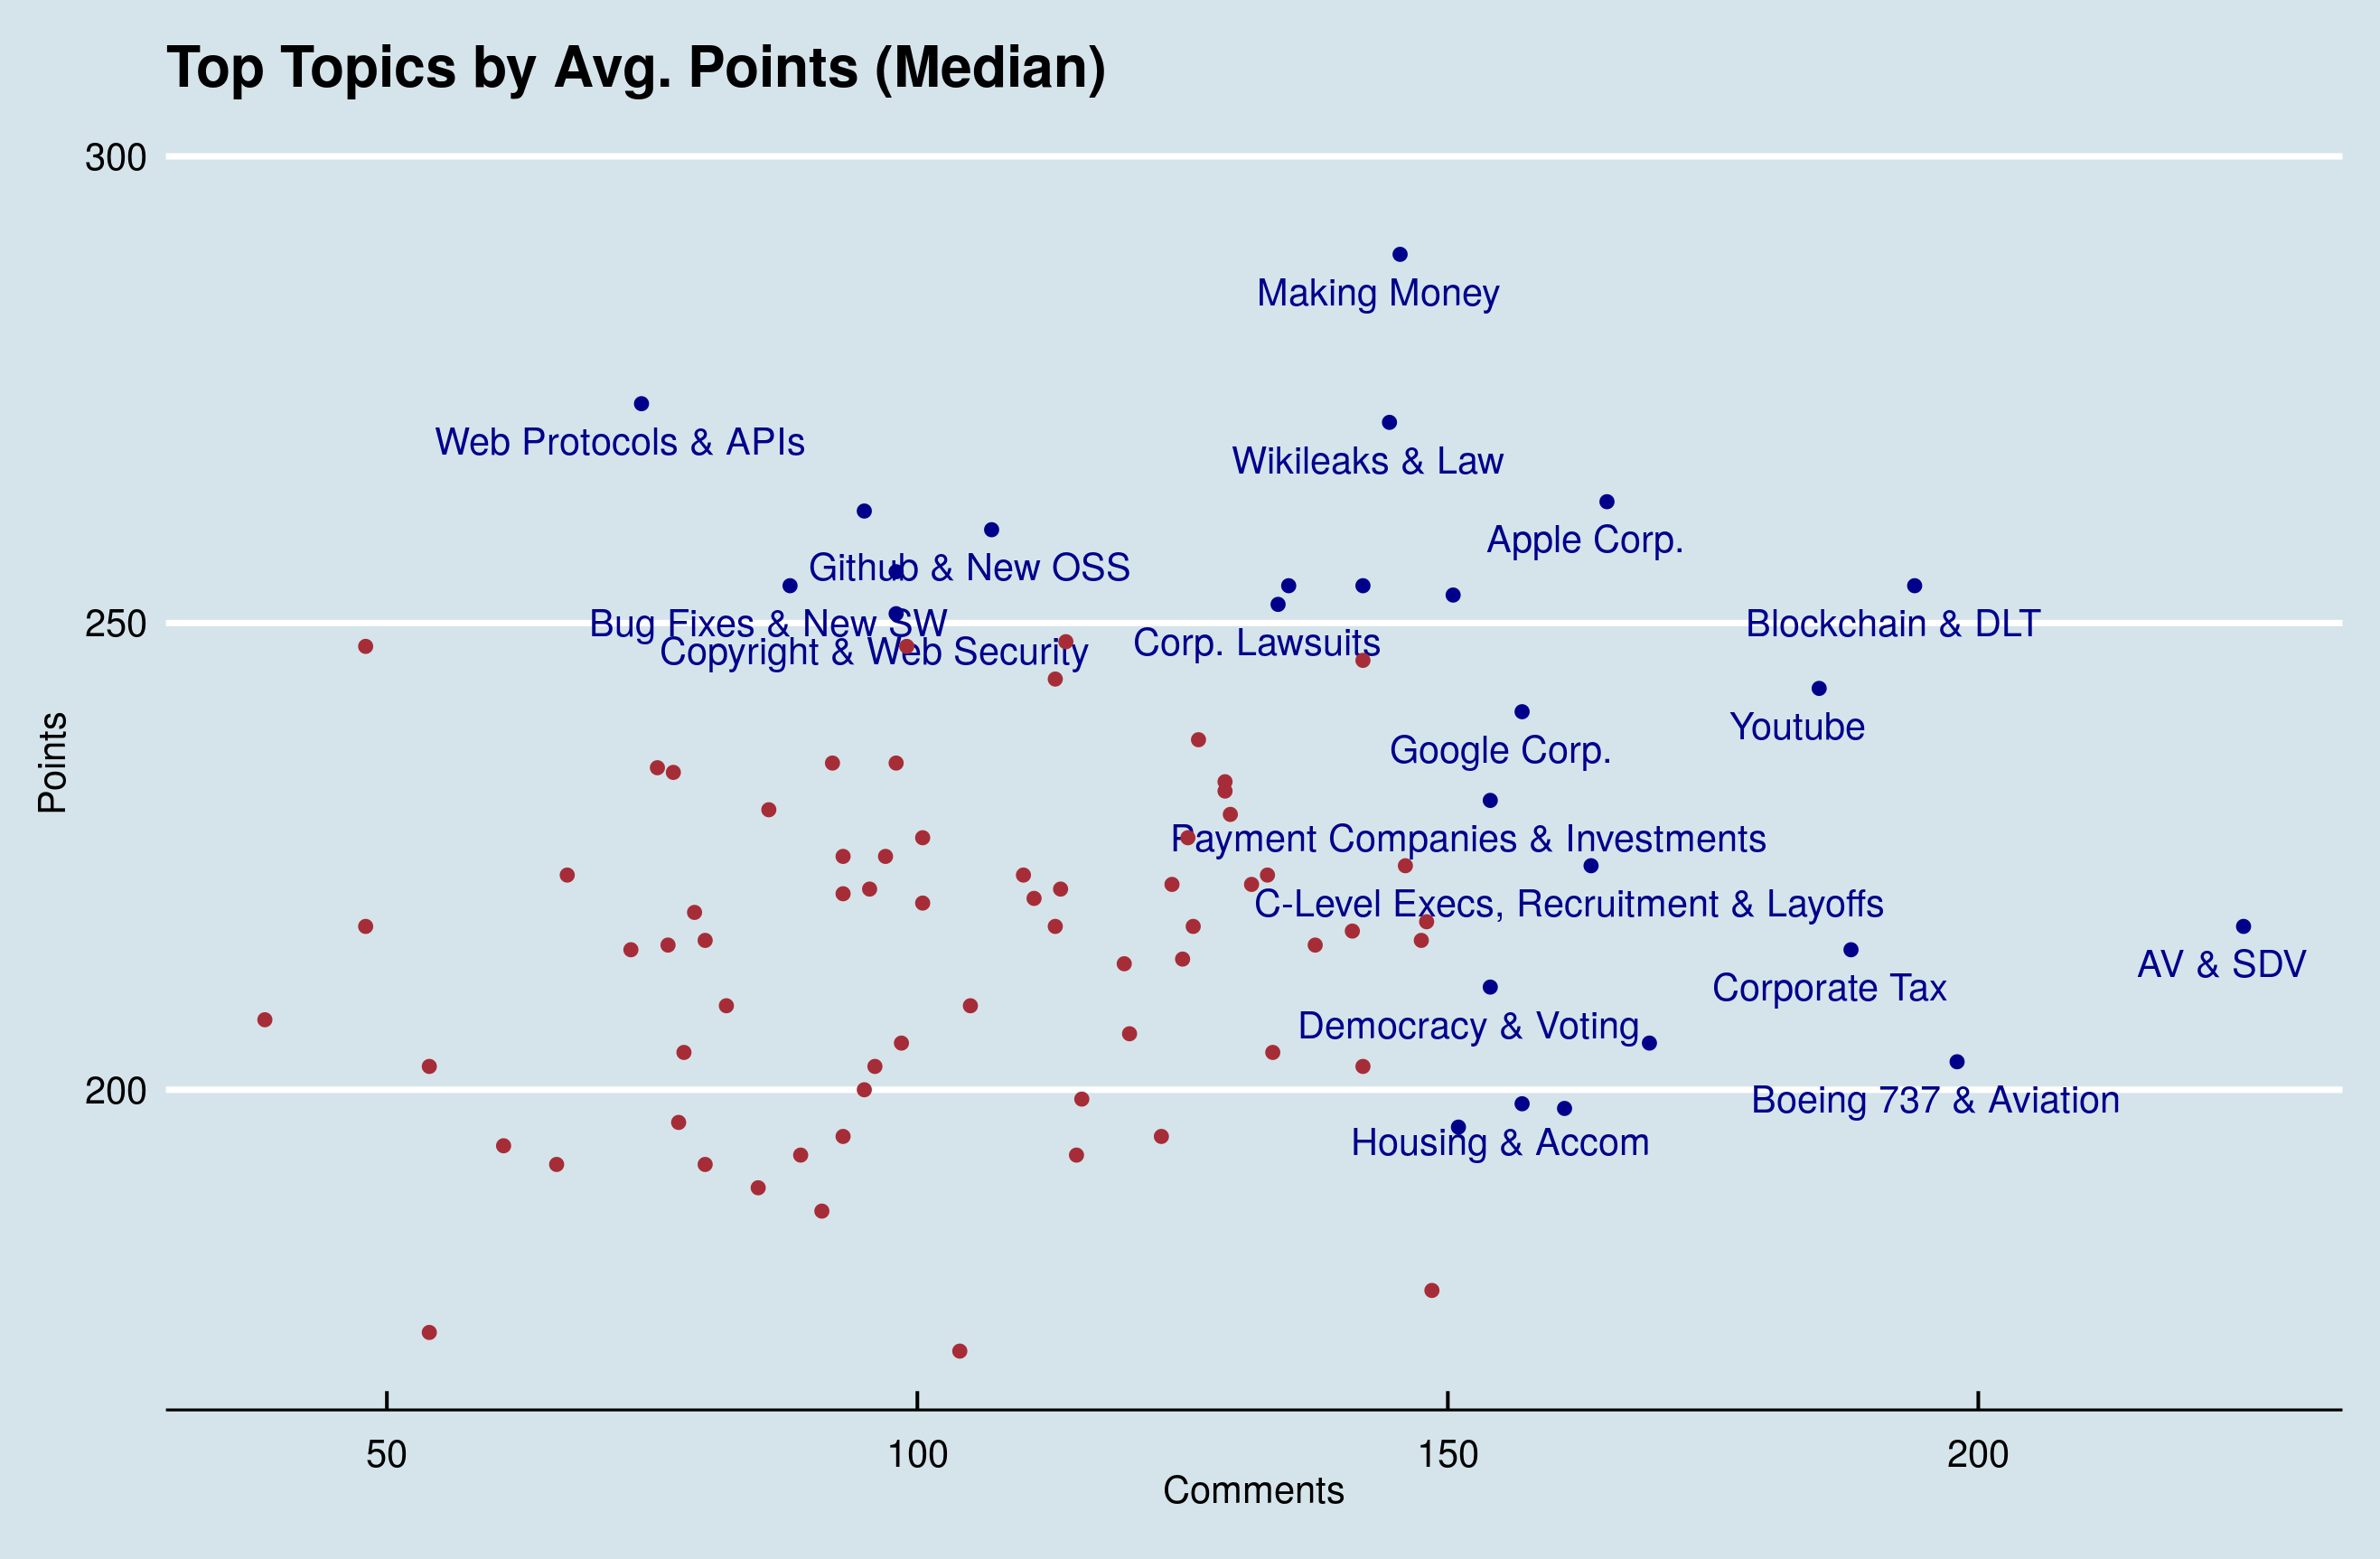
\includegraphics[scale=0.4]{img/topic_model_02_alltopics.png}}
\caption{Detected Topics by Comments and Points}
\label{fig7}
\end{figure}

A cursory view of the plot shows that the top topics are \textit{Hiring and Careers}, encompassing stories related to the workplace and the hiring process; \textit{Making Money}, related to different businesses models and their revenues; \textit{Web Protocols and APIs}, relating to web standards and news related to updates; \textit{Wikileaks and Law}, pertaining to articles about \textit{Julian Assange} and court orders; and \textit{Apple}, the multinational technology company. Such topics are indicative of the fact that Hacker News brings together startup founders and software developers.

\begin{table}[!ht]
\centering
\tiny
\begin{tabular}{lll}
\hline
Annotation            & Story Headline                                                                                                                                  & Points \\ \hline
Hiring \& Careers     & \begin{tabular}[c]{@{}l@{}}Absolute truths I unlearned \\  as junior developer (monicalent.com)\end{tabular}                                  & 1478   \\ \hline
Hiring \& Careers     & \begin{tabular}[c]{@{}l@{}}I interviewed at six top companies \\  in Silicon Valley in six days (blog.usejournal.com)\end{tabular}            & 970    \\ \hline
Hiring \& Careers     & \begin{tabular}[c]{@{}l@{}}When hiring senior engineers, you’re not buying, \\  you’re selling (hiringengineersbook.com)\end{tabular}         & 941    \\ \hline
Making Money          & How to Be Successful (blog.samaltman.com)                                                                                                       & 836    \\ \hline
Making Money          & \begin{tabular}[c]{@{}l@{}}Firefox desktop market share \\  now below 9\% (netmarketshare.com)\end{tabular}                                   & 821    \\ \hline
Making Money          & \begin{tabular}[c]{@{}l@{}}Open Source Doesn’t Make Money Because \\  It Isn’t Designed to Make Money (www.ianbicking.org)\end{tabular}       & 716    \\ \hline
Web Protocols \& APIs & \begin{tabular}[c]{@{}l@{}}Remote Code Execution on \\  Most Dell Computers (d4stiny.github.io)\end{tabular}                                  & 870    \\ \hline
Web Protocols \& APIs & HTTP headers for the responsible developer (www.twilio.com)                                                                                     & 866    \\ \hline
Web Protocols \& APIs & HTTP/3 explained (http3-explained.haxx.se)                                                                                                      & 708    \\ \hline
Wikileaks \& Law      & Julian Assange arrested in London (www.bbc.co.uk)                                                                                               & 2354   \\ \hline
Wikileaks \& Law      & \begin{tabular}[c]{@{}l@{}}U.S. Supreme Court Puts Limits on Police \\  Power to Seize Private Property (www.nytimes.com)\end{tabular}        & 1411   \\ \hline
Wikileaks \& Law      & \begin{tabular}[c]{@{}l@{}}If Software Is Funded from a Public Source, \\  Its Code Should Be Open Source (www.linuxjournal.com)\end{tabular} & 1131   \\ \hline
Apple Corp.           & Spotify to Apple: Time to Play Fair (www.timetoplayfair.com)                                                                                    & 1876   \\ \hline
Apple Corp.           & \begin{tabular}[c]{@{}l@{}}FaceTime bug lets you hear audio of person \\  you are calling before they pick up (9to5mac.com)\end{tabular}      & 1531   \\ \hline
Apple Corp.           & Apple Sign In (techcrunch.com)                                                                                                                  & 1137   \\ \hline
\\
\end{tabular}

\caption{Top stories which form part of the top voted topics}
\label{tab:topstories}
\end{table}


\subsubsection{Topic Prevalence within the Front Page}
Following a visual analysis of the top topics, we aim to answer the question: \textit{"Are there particular topics which make it more often to the front page?"} On one hand, one may consider topics in isolation, as per our prior analysis, however this does not account for the fact that topics are overlapping and inter-related. Moreover, the concept of a topic does not occur in isolation, on the contrary, a popular topic is bound to have other related popular topics. Thus we aim to detect clusters of topics, which occur more frequently together.

We do this by computing a document-topic probability covariance matrix, which displays the probability of two topics occurring together. Figure \ref{covar} shows the covariance matrix containing the distribution over log probabilities between topics, clustered hierarchically.


\begin{figure}[!ht]
\centerline{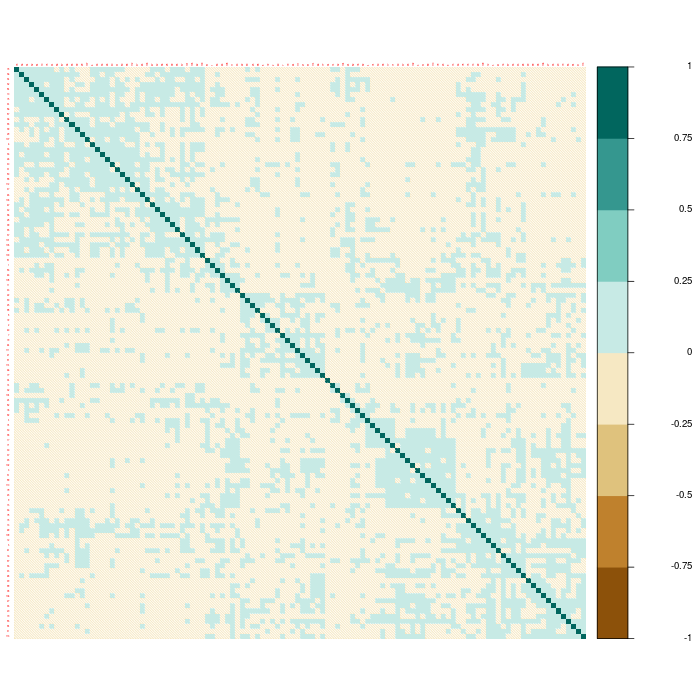
\includegraphics[scale=0.3]{img/topic_model_03_allarticles_full_SMALL.png}}
\caption{Covariance Matrix of Topics}
\label{covar}
\end{figure}

Interpreting the covariance is not a trivial exercise, however one can see that there are a number of topics which are tightly related from the density of colours. We use this visualization to detect groups of topics as clusters. Table \ref{tab:clusters} shows a table of topics which were extracted from our interpretation.

\begin{table}[!ht]
\centering
\scriptsize
\begin{tabular}{lll}
\hline
\begin{tabular}[c]{@{}l@{}}Topic\\ Id\end{tabular} & Topic Annotation                                                                                              & Cluster Name \\ \hline
11                                                 & Making Money                                                                                                 & Cluster 1    \\ \hline
15                                                 & Corporate Revenue \& Transactions                                                                            & Cluster 1    \\ \hline
37                                                 & Corporate Tax                                                                                                & Cluster 1    \\ \hline
23                                                 & C-Level Execs, Recruitment \& Layoffs                                                                        & Cluster 1    \\ \hline
3                                                  & Geopolitics                                                                                                  & Cluster 1    \\ \hline
17                                                 & Lawmaking, Policy \& Trump                                                                                   & Cluster 1    \\ \hline
43                                                 & Payment Companies \& Investments                                                                             & Cluster 1    \\ \hline
9                                                  & VC,IPOs \& Money                                                                                             & Cluster 1    \\ \hline
50                                                 & Government Surveillance                                                                                      & Cluster 1    \\ \hline
30                                                 & Demographic Statistics                                                                                       & Cluster 1    \\ \hline
51                                                 & Nosiy Topic G                                                                                                & Cluster 1    \\ \hline
48                                                 & Housing \& Accom                                                                                             & Cluster 2    \\ \hline
22                                                 & Japanese Tech.                                                                                               & Cluster 2    \\ \hline
35                                                 & Problems \& The Past & Cluster 2    \\ \hline
21                                                 & Noisy Topic B                                                                                                & Cluster 2    \\ \hline
20                                                 & Movies \& Entertainment                                                                                      & Cluster 2    \\ \hline
12                                                 & Quitting Jobs \& Toxic SV Culture                                                                            & Cluster 2    \\ \hline
27                                                 & Terrorism \& General Crime                                                                                   & Cluster 2    \\ \hline
47                                                 & Math, Simulations \& Trading                                                                                 & Cluster 3    \\ \hline
53                                                 & Functional Lagnuages                                                                                         & Cluster 3    \\ \hline
44                                                 & Noisy Topic E                                                                                                & Cluster 3    \\ \hline
6                                                  & Rust Lang.                                                                                                   & Cluster 3    \\ \hline
31                                                 & Noisy Topic C                                                                                                & Cluster 3    \\ \hline
40                                                 & Ruby Lang.                                                                                                   & Cluster 3    \\ \hline
33                                                 & Interpreted Prog. Languages                                                                                  & Cluster 3    \\ \hline
57                                                 & Concurrency \& Parallel Programming                                                                          & Cluster 3    \\ \hline
26                                                 & Fast \& Efficient Porgramming                                                                                & Cluster 3    \\ \hline
77                                                 & Nature, Animals \& Insects                                                                                   & Cluster 4    \\ \hline
113                                                & Family Issues \& Happiness                                                                                   & Cluster 4    \\ \hline
94                                                 & Chess \& Games \& Board Games                                                                                & Cluster 4    \\ \hline
85                                                 & Noisy Topic K                                                                                                & Cluster 4    \\ \hline
110                                                & Noisy Topic Q                                                                                                & Cluster 5    \\ \hline
89                                                 & Huawei \& China                                                                                              & Cluster 5    \\ \hline
58                                                 & Wikileaks \& Law                                                                                             & Cluster 5    \\ \hline
71                                                 & Corp. Lawsuits                                                                                               & Cluster 5    \\ \hline
\\
\end{tabular}
\caption{Clusters Extracted from Covariance Matrix}
\label{tab:clusters}
\end{table}

One can observe that \textit{Cluster 1} is heavily related to corporate developments, including the topics \textit{Making Money, Corporate Revenue \& Transactions, Corporate Tax} and some other generic topics relating to geopolitics and lawmaking. The second cluster, \textit{Cluster 2}, contains topics which are related to lifestyle, including \textit{Housing \& Accommodation, Toxic Workplace Culture and Movies}. \textit{Cluster 3} relates to software development niches, covering specific programming languages and techniques. 

It is interesting to note that overlapping that topic 71, pertaining to corporate lawsuits, does not fall within \textit{Cluster 1}. Moreover, we observe that our clustering method has detected many Noisy Topics - this can be attributed to the fact that the noisy topics do not focus on a single subject matter, and are likely to associated with several different documents.

Similar to our initial analysis, we plot these clusters by points and comments, in order to gain a better understanding of how the clusters rank against each other.  We observe that \textit{Cluster 1}, relating to corporate culture, generates the most activity both in terms of points and comments. However, the distribution is sparse. On the other hand, \textit{Cluster 5}, which relates to censorship and lawsuits, is similarly successful but less sparse.

\begin{figure}[!ht]
\centerline{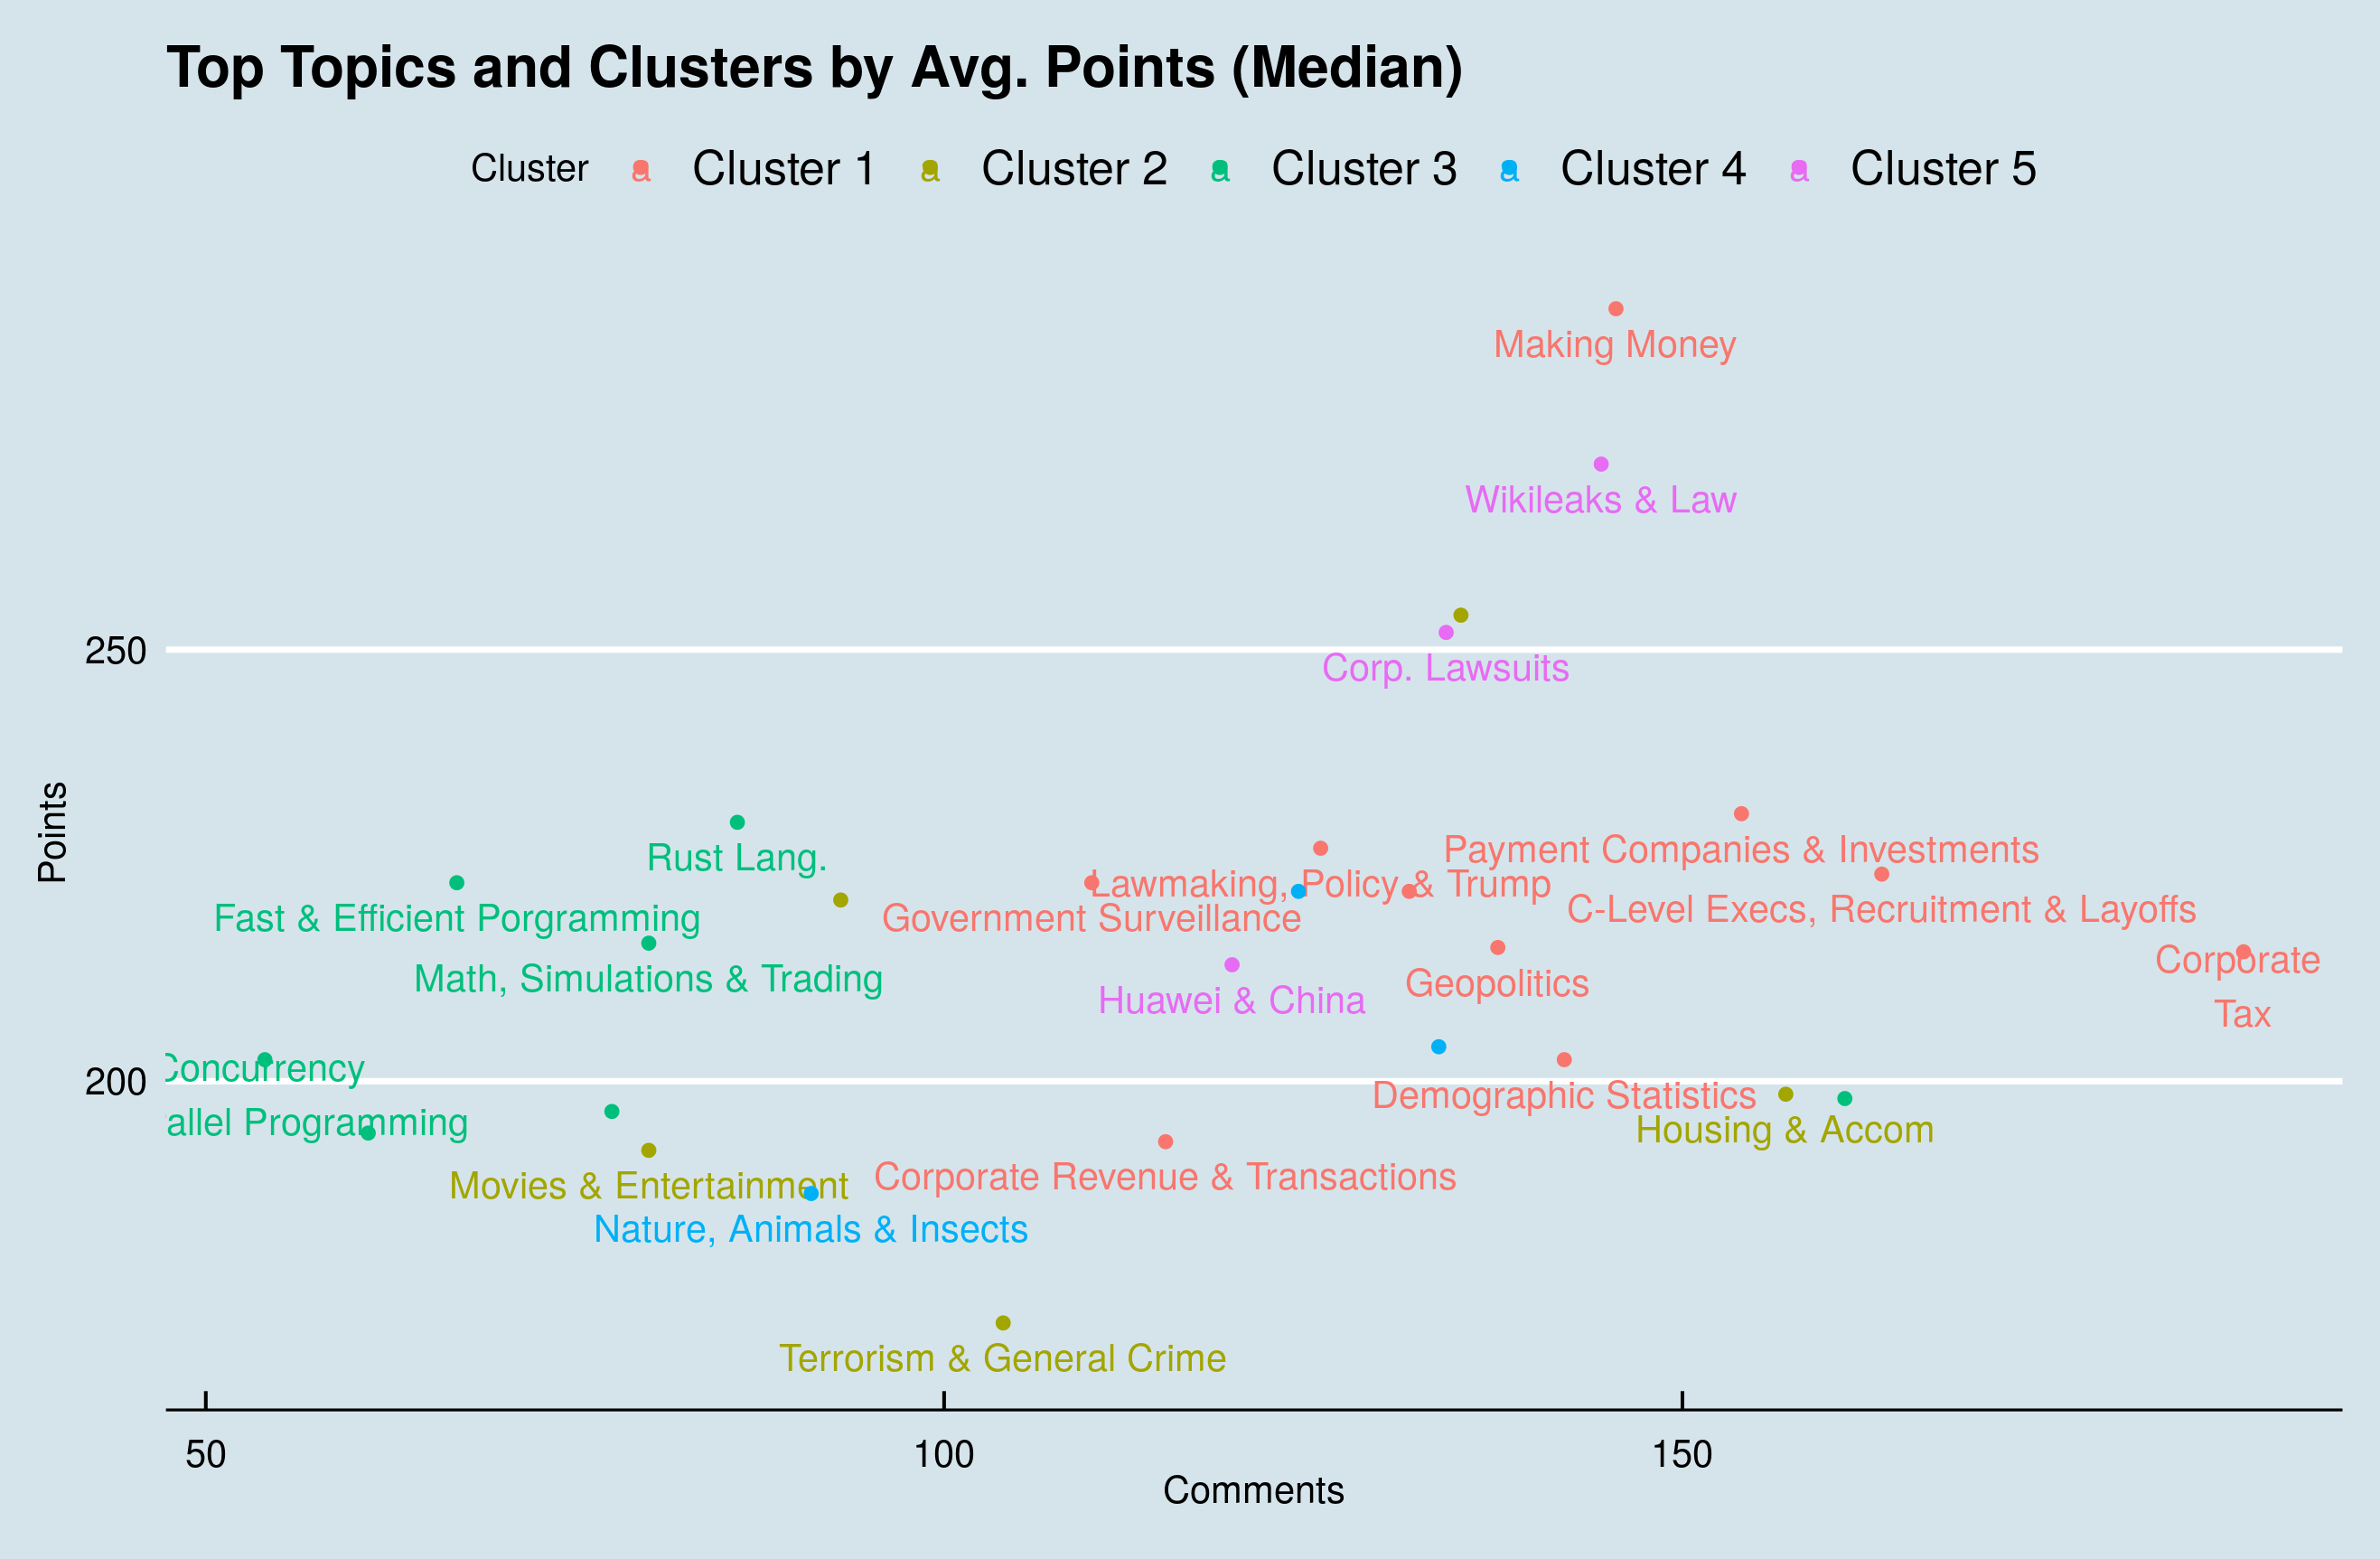
\includegraphics[scale=0.4]{img/topic_model_02_plot_clusters.png}}
\caption{Top Clustered Topics appearing on the Front Page}
\label{covar}
\end{figure}

The cluster relating to niche programming concepts tends is least discussed, but similarly successful to other clusters. It is also the most concentrated cluster within the plot. We also observe that clusters with more controversial topics, such as layoffs and tax, are more discussed - this is indicative of the fact that divisive topics create confrontation, and thus more dialogue. 

We conclude that while our analysis shows several topic groups which are most likely to make it to the front page, topics relating to corporate entities, generating revenue, lawmaking, Wikileaks and niche software development are most represented on the front page. 

\subsubsection{Topic Over-representation within the top post}
The above observations hold true for the whole front page of Hacker News, having detected topics from stories ranked one through thirty. Next, we aim to evaluate whether certain topics are over-represented within the top post. We pose the null hypothesis:
 
$H_{0}$ : \textit{"Achieving the top rank from within the front page is unrelated to the story topic."} 

We first perform a Chi-Square test between two categorical values: the topic name, and the binned rank, which shows a one if a story was in the top post, and zero if the story was shown in any other rank. A \textit{p-value} of 0.002634, which falls under the 0.05 critical value is obtained. 

One must note that the probability obtained with this test is remarkably small, this is primarily due to the reason that the frequencies are relatively small - thus our test may be inconsistent. Thus we perform an additional statistical test, a One-Way ANOVA Test. Our One-Way ANOVA test between a nominal value, the story rank, and a categorical value, the topic. Table \ref{tab:anova} shows the results of our One-Way ANOVA test, resulting in a \textit{p-value} which also falls under the critical value of 0.05.

\begin{table}[!ht]
\centering
\scriptsize
\begin{tabular}{llllll}
\hline
               & Df    & Sum Sq & Mean Sq & F value & Pr(\textgreater{}F) \\ \hline
Topic          & 113   & 16588  & 146.80  & 1.996   & 2.97e-09            \\ \hline
Residuals      & 5825  & 428417 & 73.55   &         &                     \\ \hline
Signifc. codes & 0.001 & 0.01   & 0.05    & 0.1     & 1                   \\ \hline
\\
\end{tabular}
\caption{One-Way Anova Test between Topics (Categorical) and Rank (Nominal)}
\label{tab:anova}
\end{table}

We reject the null hypothesis $H_{0}$ with a \textit{p-value} of 0.002634, which falls under the 0.05 critical p-value. Therefore we conclude that there is strong evidence that indicates that the top rank is \textit{highly} dependent on the topics present, rejecting the null hypothesis. 

Thus we are able to conclude that some\textbf{topics are indeed over-represented within the top post} - we now investigate which topics are represented within the top post.

\begin{figure}[!ht]
\centerline{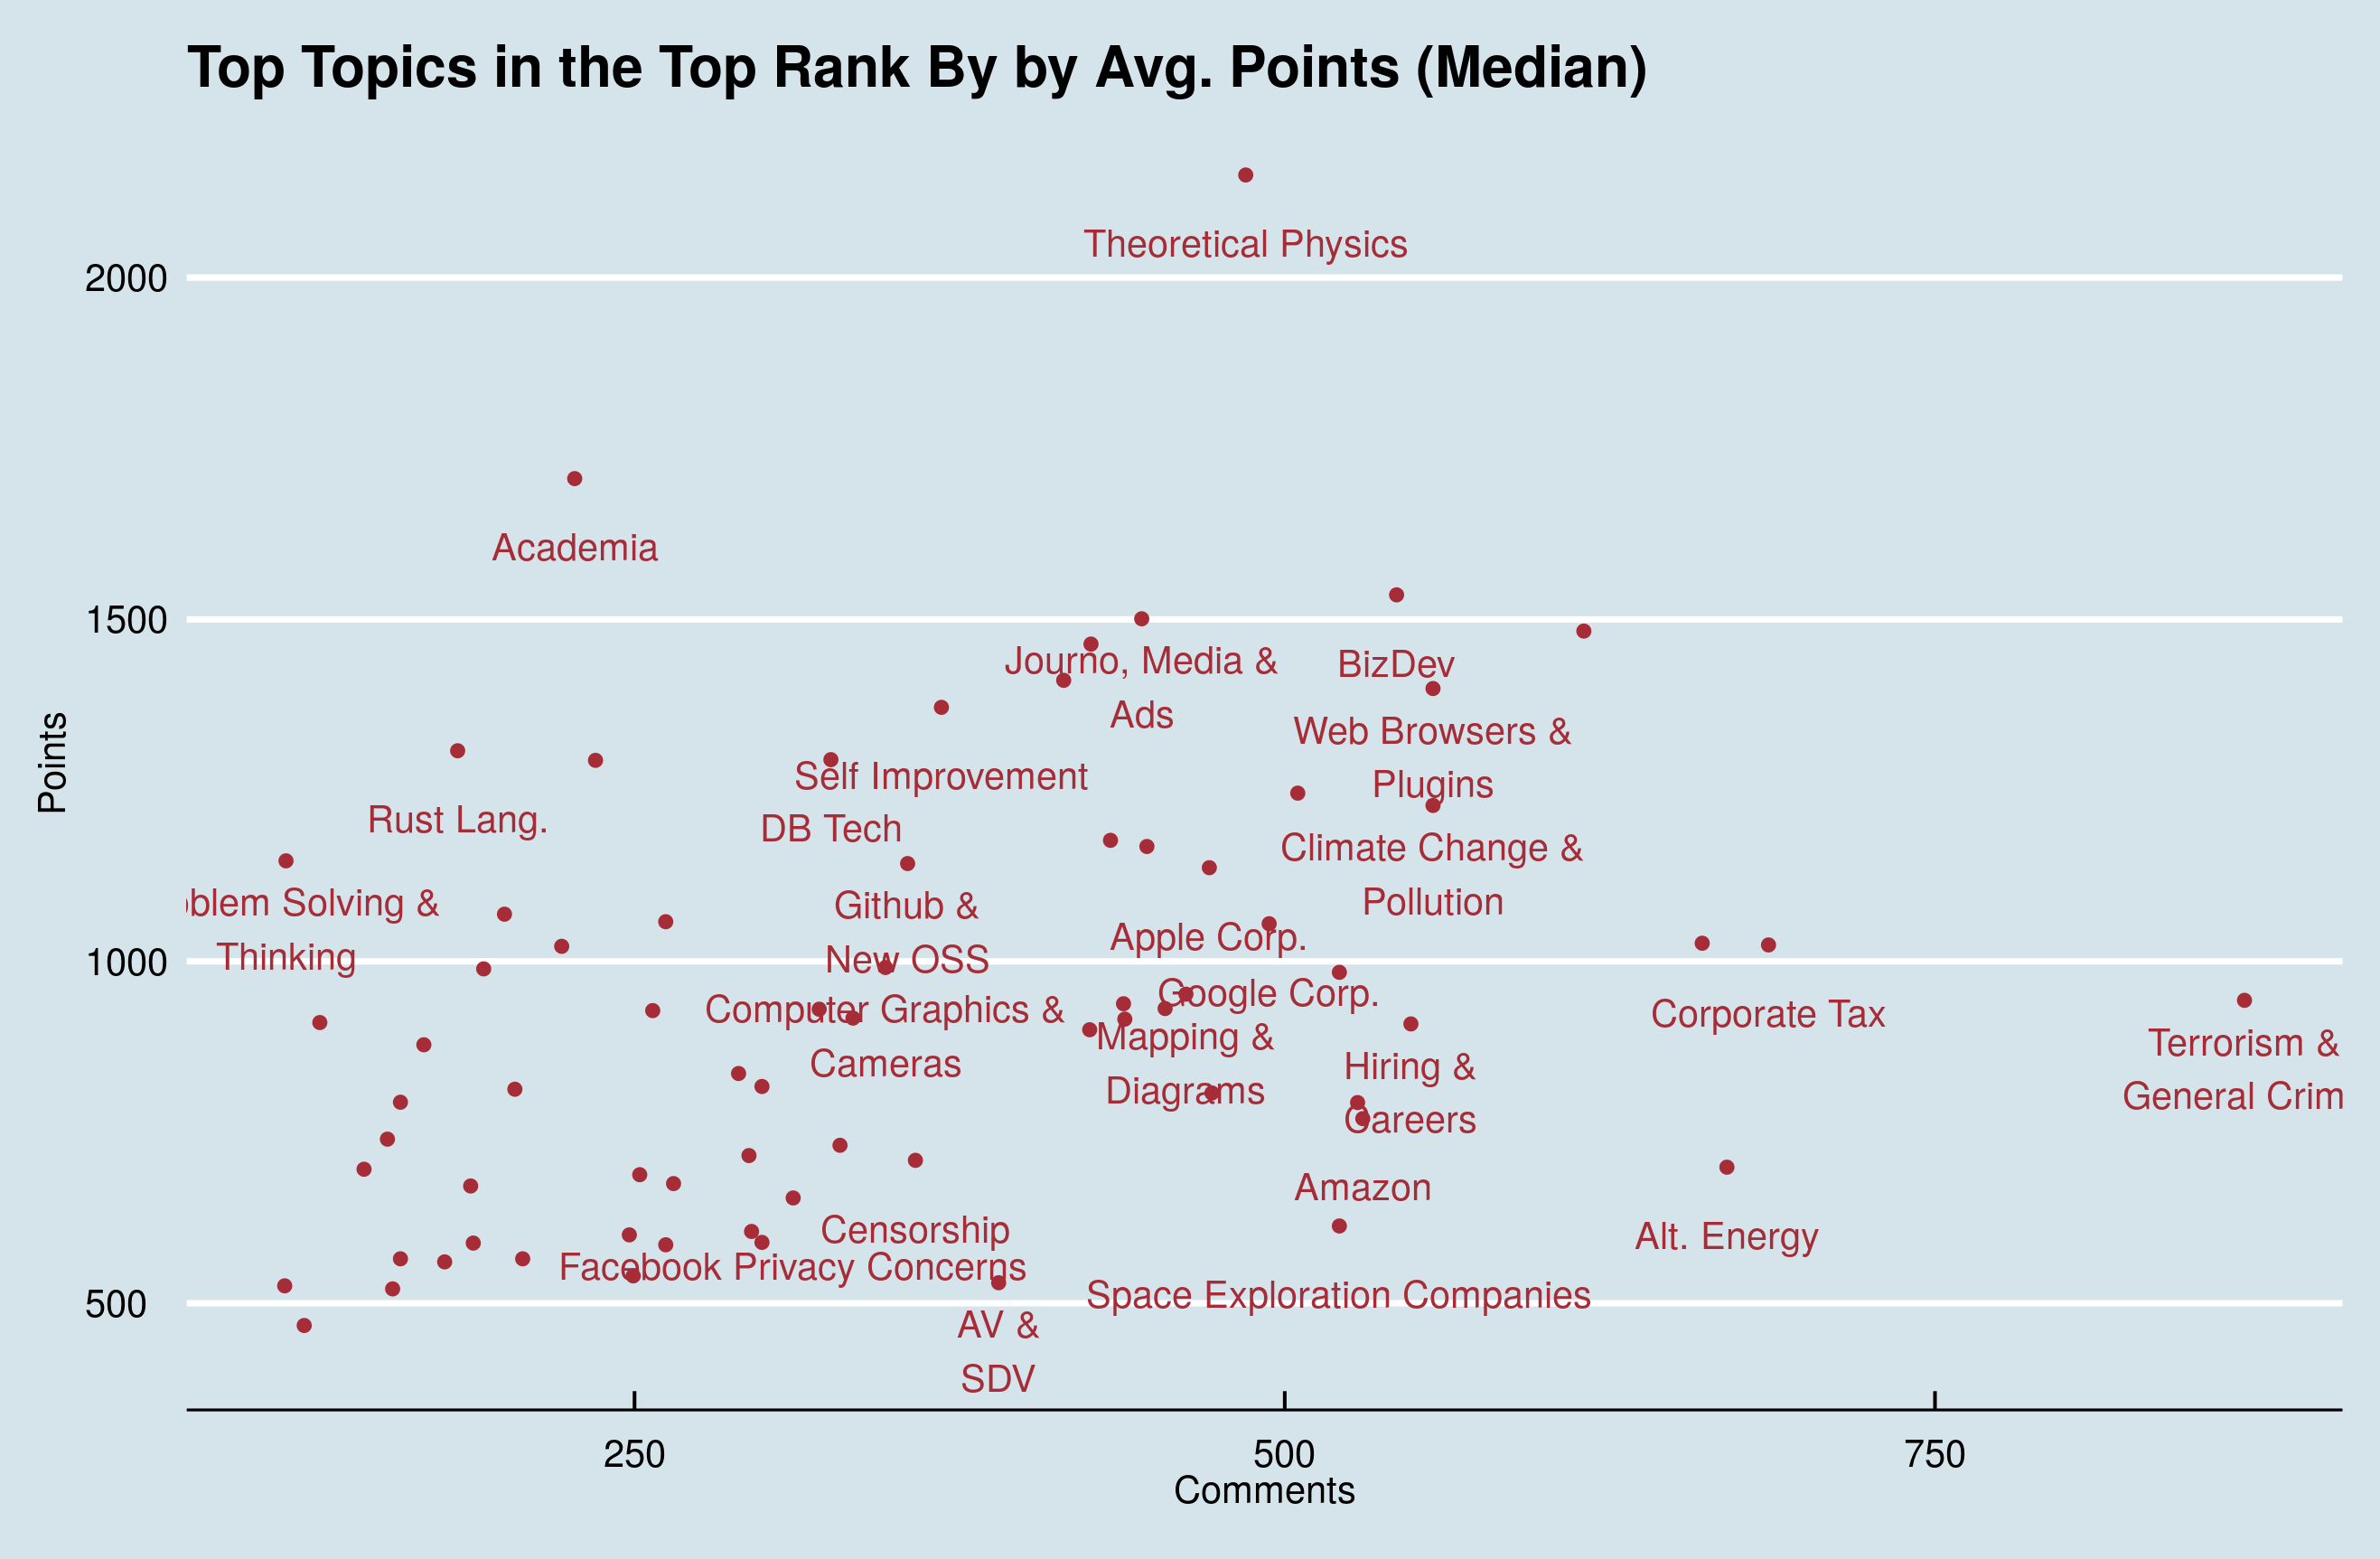
\includegraphics[scale=0.4]{img/topic_model_02_top_post_ranking_med.png}}
\caption{Top Topics by Median Points}
\label{toptopicsmedpoints}
\end{figure}

Filtering the topics by the top rank, and selecting the top topics by median post shows a different set of top topics than observed across the full ranking - the only topic retained is related to Wikileaks and Law. The top ranked topic of all time is \textit{Theoretical Physics}, due to the heavily up-voted article on the first ever image of a black hole. Table \ref{toprank:toptopics} shows the list of top topics within the top rank using this method, while figure \ref{toptopicsmedpoints} shows a scatter plot of these topics.

\begin{table}[!ht]
\centering
\tiny
\begin{tabular}{lll}
\hline
Topic                                                                  & Story                                                                                                                                                    & Points \\ \hline
\begin{tabular}[c]{@{}l@{}}Theoretical \\ Physics\end{tabular}         & \begin{tabular}[c]{@{}l@{}}Unveiling the first-ever image of a\\  black hole {[}video{]} \\ (www.youtube.com)\end{tabular}                               & 2150   \\ \hline
Academia                                                               & \begin{tabular}[c]{@{}l@{}}UC terminates subscriptions with \\ Elsevier in push for open access \\ (www.universityofcalifornia.edu)\end{tabular}         & 1706   \\ \hline
BizDev                                                                 & \begin{tabular}[c]{@{}l@{}}Start with a Website, Not a Mobile App\\  (www.atrium.co)\end{tabular}                                                        & 1536   \\ \hline
\begin{tabular}[c]{@{}l@{}}Journo, Media \\ \& Ads\end{tabular}        & \begin{tabular}[c]{@{}l@{}}No Thank You, Mr. Pecker \\ (medium.com)\end{tabular}                                                                         & 2400   \\ \hline
\begin{tabular}[c]{@{}l@{}}Journo, Media \\ \& Ads\end{tabular}        & \begin{tabular}[c]{@{}l@{}}Bezos Investigation Says the Saudis \\ Obtained His Private Data \\ (www.thedailybeast.com)\end{tabular}                      & 602    \\ \hline
\begin{tabular}[c]{@{}l@{}}Containers, \\ Orch \& Cloud\end{tabular}   & \begin{tabular}[c]{@{}l@{}}Please do not attempt to \\ simplify this code \\ (github.com)\end{tabular}                                                   & 1483   \\ \hline
\begin{tabular}[c]{@{}l@{}}Malicious Company \\ Behaviour\end{tabular} & \begin{tabular}[c]{@{}l@{}}Google Tried to Patent My Work \\ After a Job Interview\\ (patentpandas.org)\end{tabular}                                     & 1757   \\ \hline
\begin{tabular}[c]{@{}l@{}}Malicious Company \\ Behaviour\end{tabular} & \begin{tabular}[c]{@{}l@{}}Apps intended for kids may  \\ not include third-party advertising\\ or analytics \\ (developer.apple.com)\end{tabular} & 1171   \\ \hline
Noisy Topic R                                                          & \begin{tabular}[c]{@{}l@{}}I made a smart watch from scratch \\ (m.imgur.com)\end{tabular}                                                               & 1431   \\ \hline
\begin{tabular}[c]{@{}l@{}}Wikileaks \\ \& Law\end{tabular}            & \begin{tabular}[c]{@{}l@{}}Julian Assange arrested in London \\ (www.bbc.co.uk)\end{tabular}                                                             & 2354   \\ \hline
\begin{tabular}[c]{@{}l@{}}Wikileaks \\ \& Law\end{tabular}            & \begin{tabular}[c]{@{}l@{}}U.S. Supreme Court Puts Limits on \\ Police Power to Seize Private Property \\ (www.nytimes.com)\end{tabular}                 & 1411   \\ \hline
\begin{tabular}[c]{@{}l@{}}Wikileaks \\ \& Law\end{tabular}            & \begin{tabular}[c]{@{}l@{}}Justice Department Is Preparing Antitrust \\ Investigation of Google (www.wsj.com)\end{tabular}                               & 867    \\ \hline
\begin{tabular}[c]{@{}l@{}}Web Browsers \\ \& Plugins\end{tabular}     & \begin{tabular}[c]{@{}l@{}}Switch from Chrome to Firefox \\ (www.mozilla.org)\end{tabular}                                                               & 3246   \\ \hline
\begin{tabular}[c]{@{}l@{}}Web Browsers \\ \& Plugins\end{tabular}     & \begin{tabular}[c]{@{}l@{}}A Conspiracy to Kill IE6 \\ (blog.chriszacharias.com)\end{tabular}                                                            & 2141   \\ \hline
\begin{tabular}[c]{@{}l@{}}Web Browsers \\ \& Plugins\end{tabular}     & \begin{tabular}[c]{@{}l@{}}Google to restrict modern ad blocking \\ Chrome extensions to enterprise users \\ (9to5google.com)\end{tabular}               & 2057   \\ \hline
Self Improvement                                                       & \begin{tabular}[c]{@{}l@{}}Ask HN: What books changed the way \\ you think about almost everything?\end{tabular}                                         & 1905   \\ \hline
Self Improvement                                                       & \begin{tabular}[c]{@{}l@{}}A guide to difficult conversations \\ (medium.dave-bailey.com)\end{tabular}                                                   & 1782   \\ \hline
Self Improvement                                                       & \begin{tabular}[c]{@{}l@{}}Why isn't the internet \\ more fun and weird? \\ (jarredsumner.com)\end{tabular}                                              & 1495   \\ \hline
\\
\end{tabular}
\caption{Top Ten Topics in the Top Post by Median Points}
\label{toprank:toptopics}
\end{table}

\begin{figure}[!ht]
\centerline{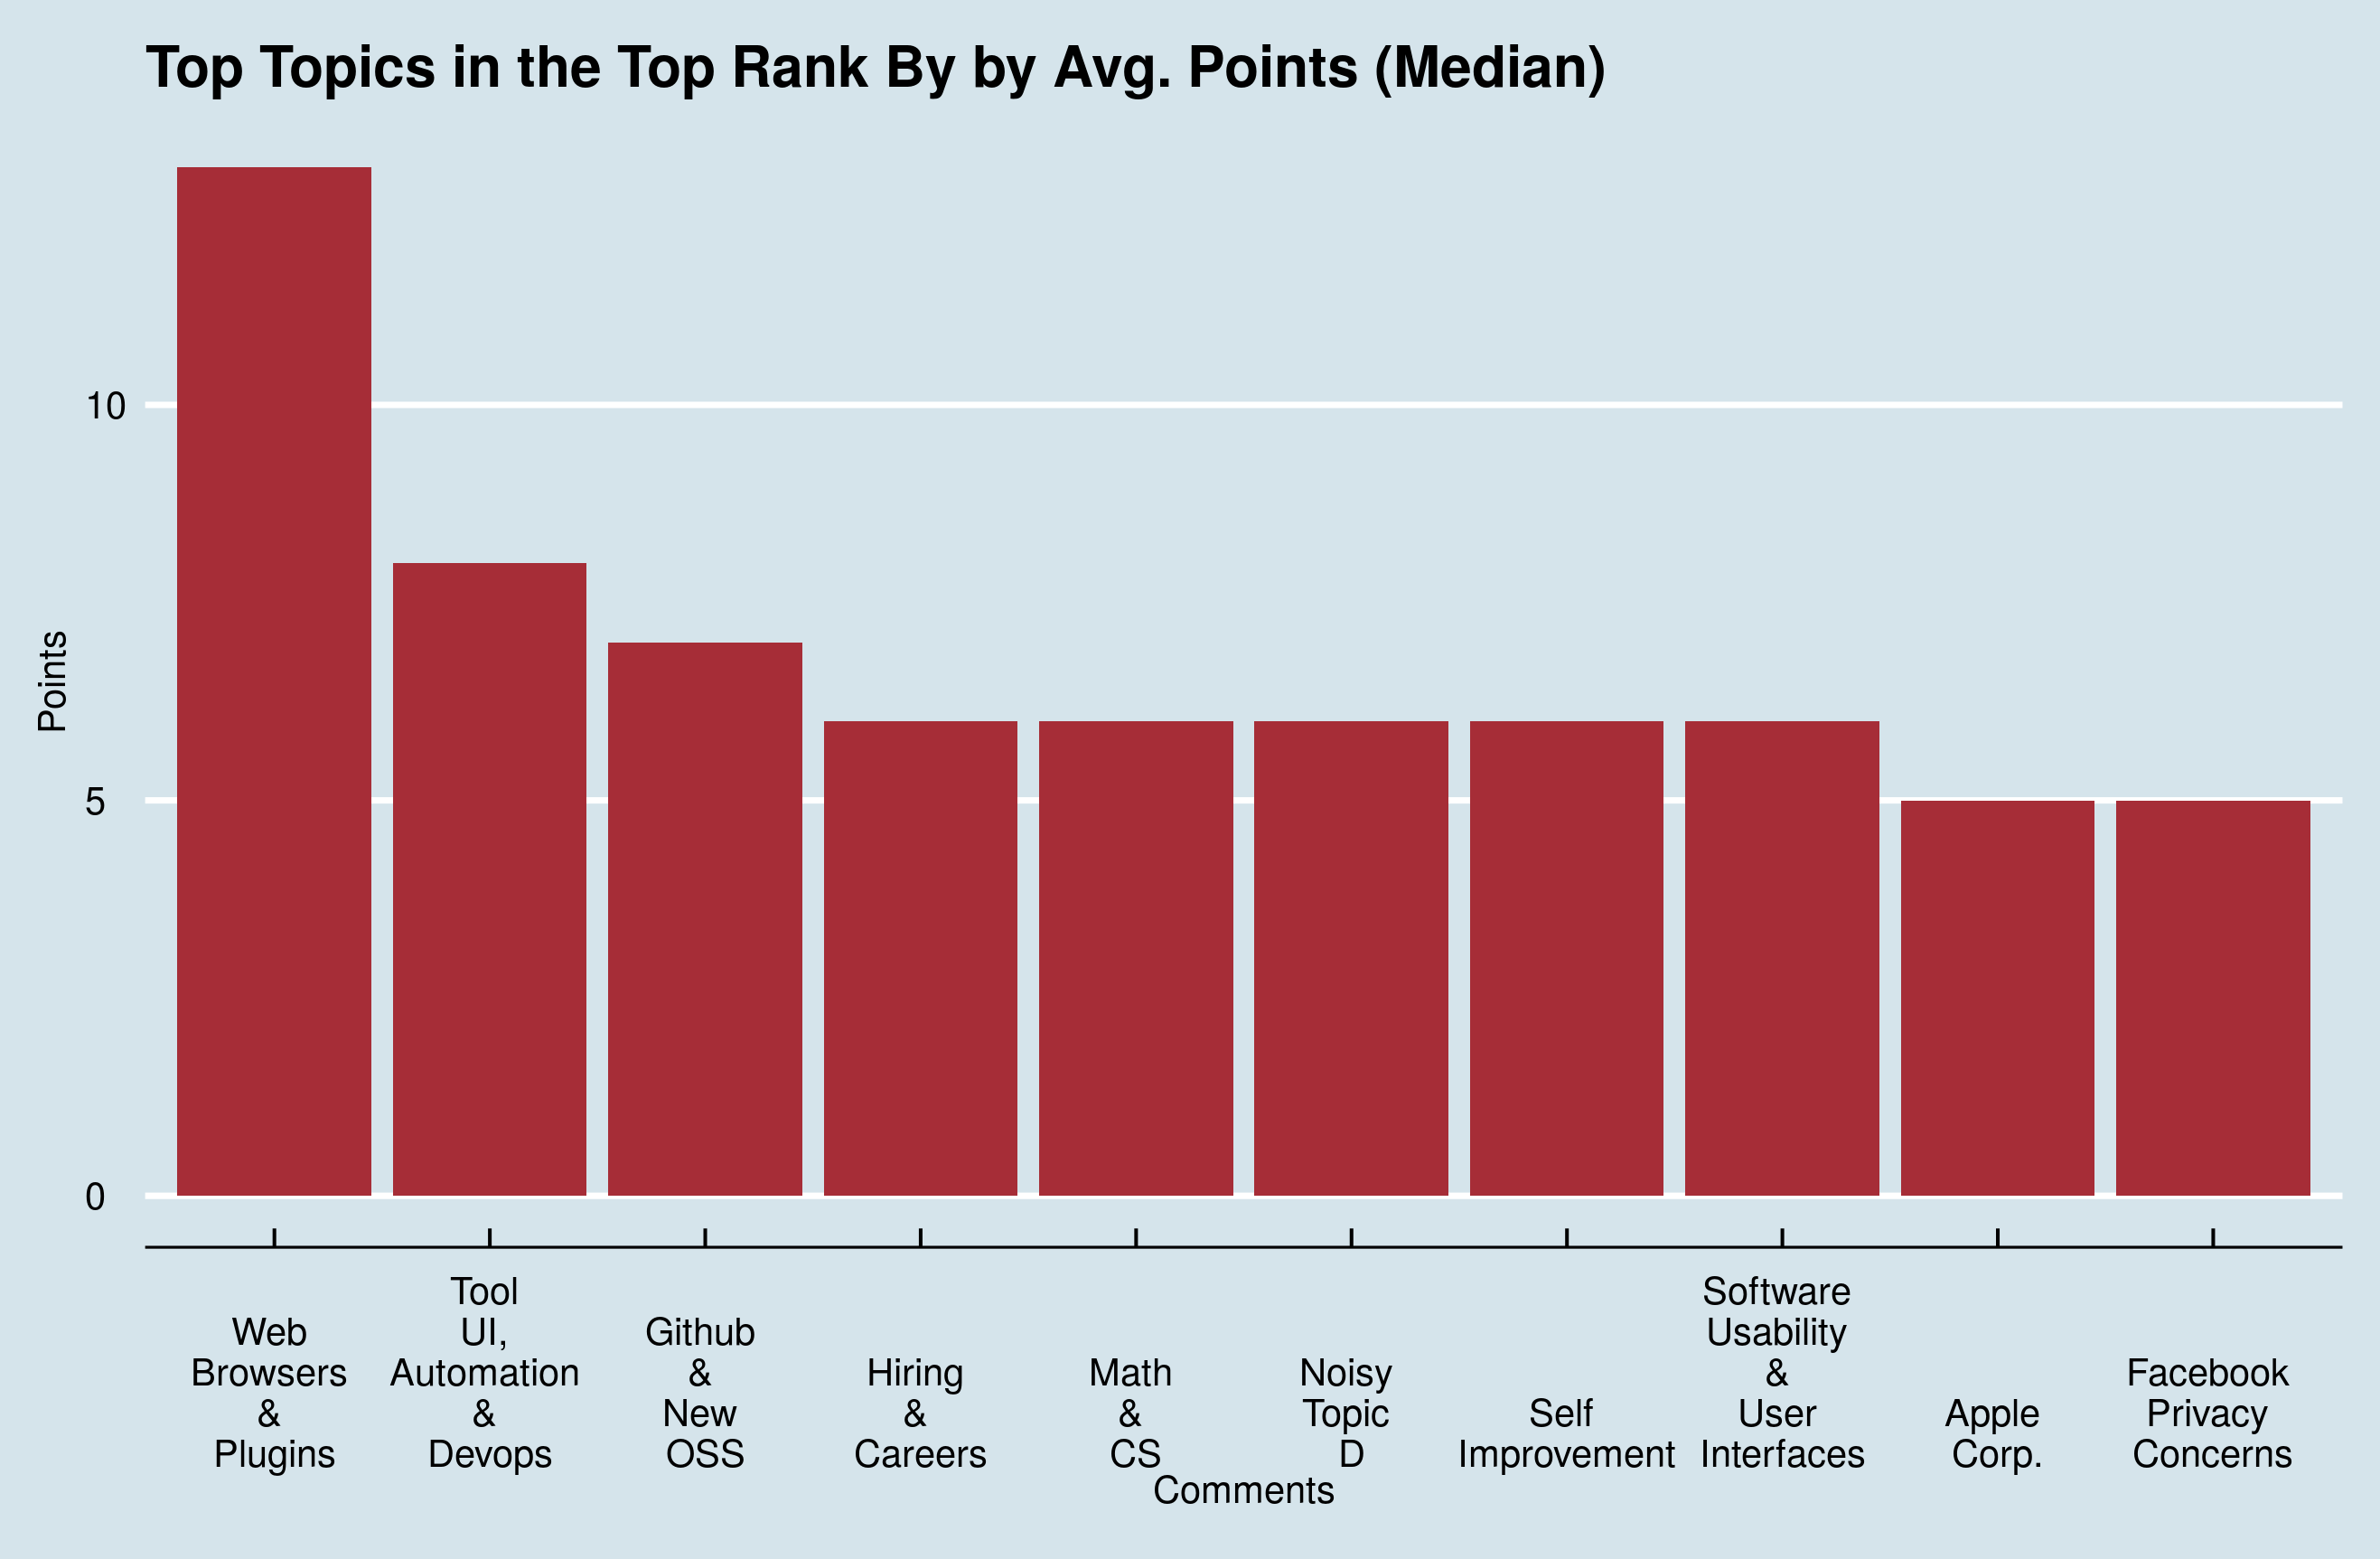
\includegraphics[scale=0.4]{img/topic_model_02_toprank_freqtabviz.png}}
\caption{Topic Occurance in Top Post}
\label{freqviz_toprank}
\end{figure}

We note that the top topics within the top rank tend to have a negative spin to them, relating to scandals, malicious company behavior and restrictions. However, one must note that this selection is highly prone to outliers. In fact, some of the top topics shown only have a one or two posts. This is perhaps due to the nature of the top post, thus we instead plot the \textit{frequency} of topic occurrence within the top post.

Figure \ref{freqviz_toprank} and table \ref{tab:tab_toprank} show us that \textit{Web Browsers \& Plugins} is most likely to occur in the top rank, with a significantly higher probability than other topics. 

In this analysis, we showed that some topics are indeed over-represented within the top rank, giving examples as to what these topics cover. Thus, we conclude that \textbf{some topics occur more often than others on the front page} and \textbf{some topics are over-represented within the top rank}. We summarize and elaborate on these key-findings in our conclusion. 

\begin{table}[!ht]
\centering
\begin{tabular}{lll}
\hline
Topic                                                                            & Frequency & Probability \\ \hline
\begin{tabular}[c]{@{}l@{}}Web Browsers \\ \& Plugins\end{tabular}               & 13        & 0.0660      \\ \hline
\begin{tabular}[c]{@{}l@{}}Tool UI, Automation \\ \& Devops\end{tabular}         & 8         & 0.0406      \\ \hline
Github \& New OSS                                                                & 7         & 0.0355      \\ \hline
Hiring \& Careers                                                                & 6         & 0.0305      \\ \hline
Math \& CS                                                                       & 6         & 0.0305      \\ \hline
Noisy Topic D                                                                    & 6         & 0.0305      \\ \hline
Self Improvement                                                                 & 6         & 0.0305      \\ \hline
\begin{tabular}[c]{@{}l@{}}Software Usability \\ \& User Interfaces\end{tabular} & 6         & 0.0305      \\ \hline
Apple Corp.                                                                      & 5         & 0.0254      \\ \hline
\begin{tabular}[c]{@{}l@{}}Facebook Privacy \\ Concerns\end{tabular}             & 5         & 0.0254      \\ \hline
\\
\end{tabular}
\caption{Top five Topics within the Top Rank by Probability}
\label{tab:tab_toprank}
\end{table}


\section{Conclusion}

Our analysis concludes that some topics are more prevalent than others on the Hacker News front page, and within the front page, certain topics are over-represented within the top post. Our key observations regarding the Hacker News front page are as follows:
\begin{enumerate}
\item The points a story receives and the comments a story receives are positively correlated, with a moderately to strong correlation and Pearson's R of 0.6.
\item Stories posted between 2pm and 7pm, and stories posted on weekdays tend to rank higher than others.
\item Certain topics tend to be over-represented on the front page. These include topics related to companies and revenue growth, such as making money, corporate transactions, corporate tax, recruitment and policy; topics relating to programming niches such as Rust programming, Ruby programming, concurrency and parallel programming and interpreted languages; and topics relating to lifestyle such as housing, movies and entertainment, job mobility and workplace culture. 
\item We reject the null hypothesis $H_{0}$, which holds that achieving the top rank from within the front page is unrelated to the story topic, with a p-value of 0.002634, showing that there is strong evidence that indicates that the top rank is highly dependent on the topics it represents. Stories related to Web Browsers, such as Mozilla Firefox and Google Chrome, are over-represented within the top post.
\end{enumerate}

The findings presented are the result of a topic detection process using Latent Dirichlet Analysis. A total of 114 topics were detected front page data spanning from the data collected, these topics were manually annotated and evaluated. Our evaluation process concluded that 18 of the 114 topics (15.8\%) were identified as noisy, representing no discernable human-identifiable topic. Noisy topics mainly resulted from source pages which were not extracted correctly, due to pay-walls or scraping prevention mechanisms or pages which were not adequately cleaned. In other cases, some noisy topics contained conceptually similar articles spanning too generic a range to discern the common topic without reading the full source. The latter topics could not be justifiably marked as quality topics. Nonetheless, we conclude that the topic detection process was successful for the purposes of our analysis.

We attribute this success mainly to good decisions within our data cleaning process. In particular, the decision to represent articles by their \textit{noun phrases} and \textit{verb phrases} proved to be very effective.

Our analysis for investigating topic representation is based on the covariance matrix drawn from the topic model. We note that interpreting a large covariance matrix is a non-trivial task, and future work on the hierarchical clustering performed could render better quality topic clusters.

Lastly, our analysis for investigating over-representation within the top post resulted in a very low \textit{p-value} for both \textit{chi-squared} test and \textit{one-way ANOVA}. We note that in the case of the \textit{chi-squared} test, the p-value may not be entirely reliable mainly due to the low-frequencies present within the data\cite{test:yates}. 

We considered calculating correlation with a logistic regression, however we observed that this does not offer any significant advantages over a chi-squared test. Moreover, an alternative Fisher's Exact Test\cite{test:fisher} \cite{test:comparison} provided similar results. Nonetheless, the fact that both our \textit{chi-squared test}, which solely draws from the top rank, and the ANOVA test, which draws nominal values for all ranks, rendered similar results. This final observation increases our confidence in the results.

Further work may include investigating the seasonality of the detected topics, augmenting the LDA model with thread comments, and excluding corporate announcements. Such suggestions may serve to further corroborate our findings, and better capture the spirit of Hacker News.


\bibliography{report-references} 
\bibliographystyle{ieeetr}

\newpage
%\includepdf[pages=1,pagecommand={},width=\textwidth]{Plagiarism_Declaration_Form_Signed.pdf}

\end{document}
